\chapter{系统设计}
\section{数据流程图}
\subsection{顶层图}
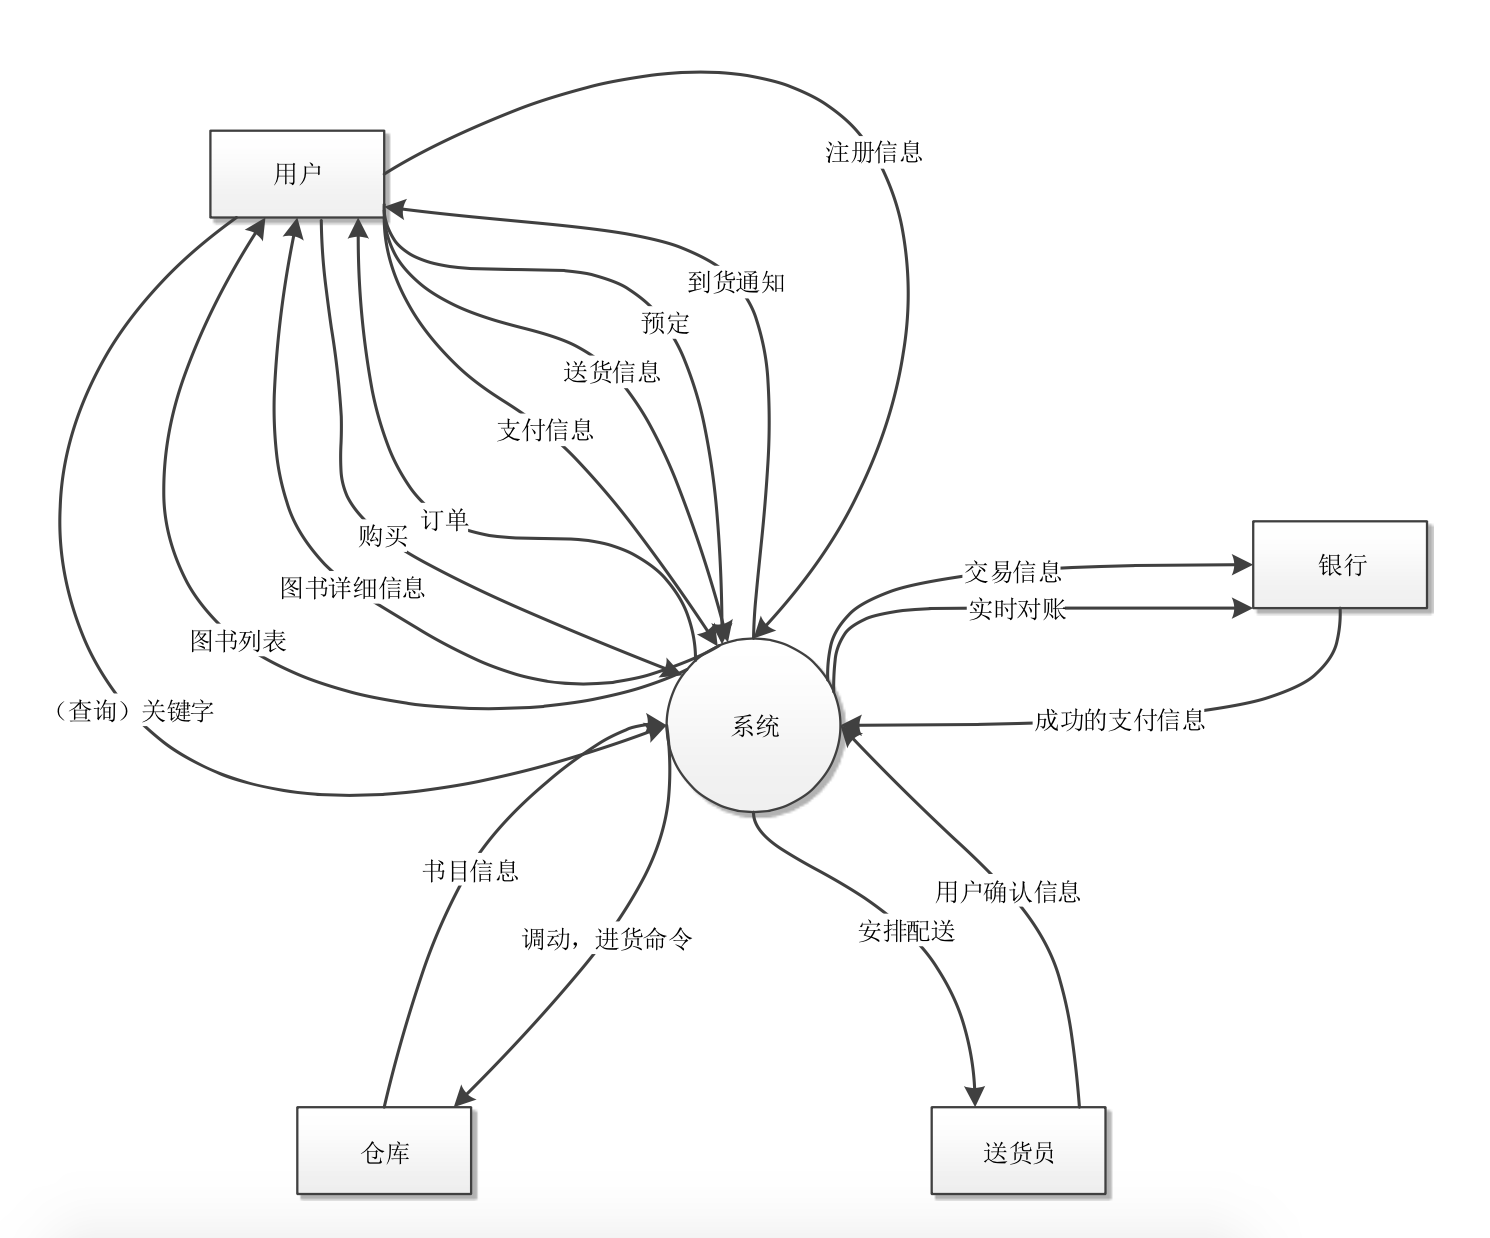
\includegraphics{img/0.png}
\subsection{0层图}
\subsubsection{用户信息管理}
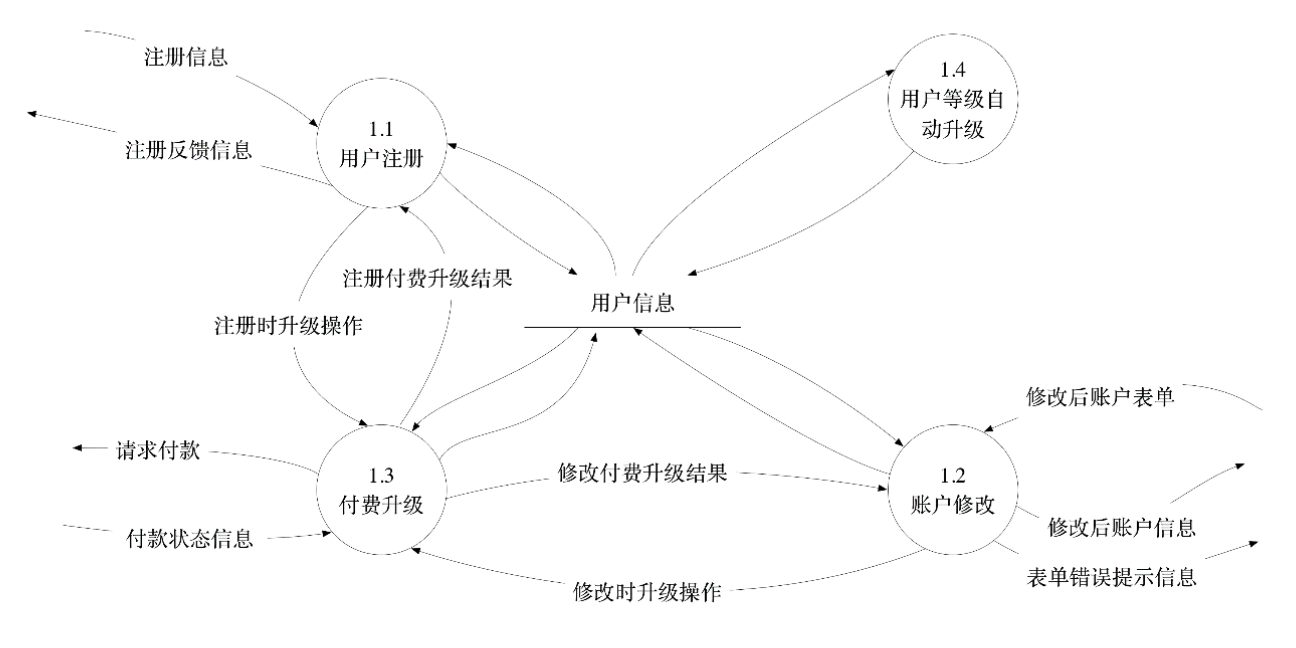
\includegraphics{img/1.png}
\paragraph{用户注册}
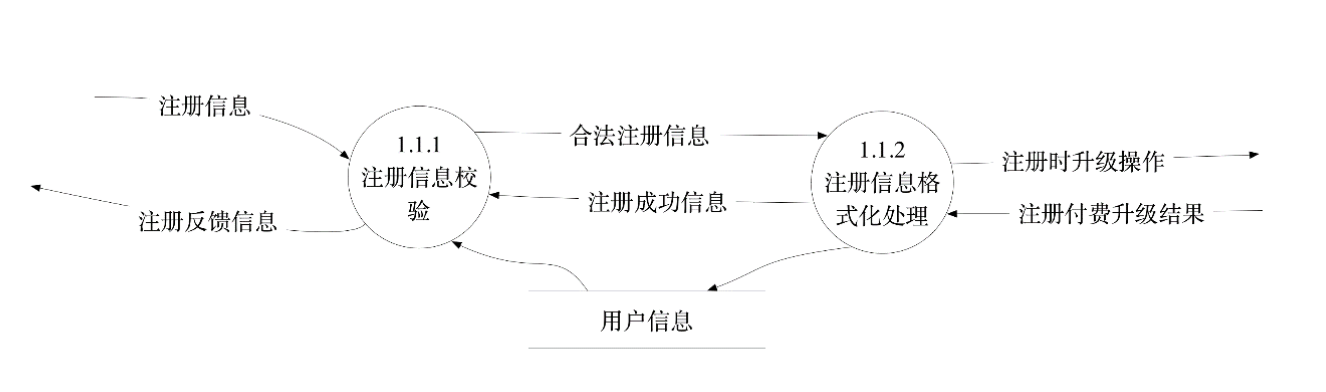
\includegraphics{img/1.1.png}
\paragraph{用户修改}
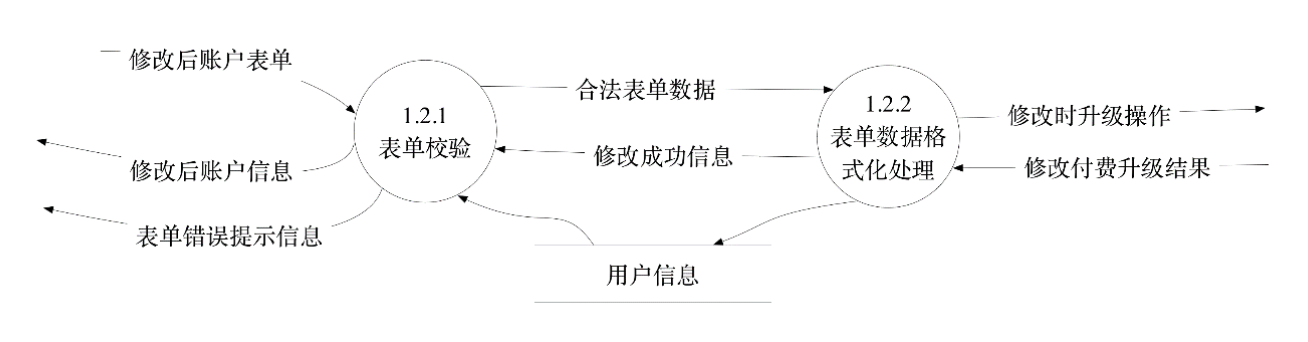
\includegraphics{img/1.2.png}
\paragraph{付费升级}
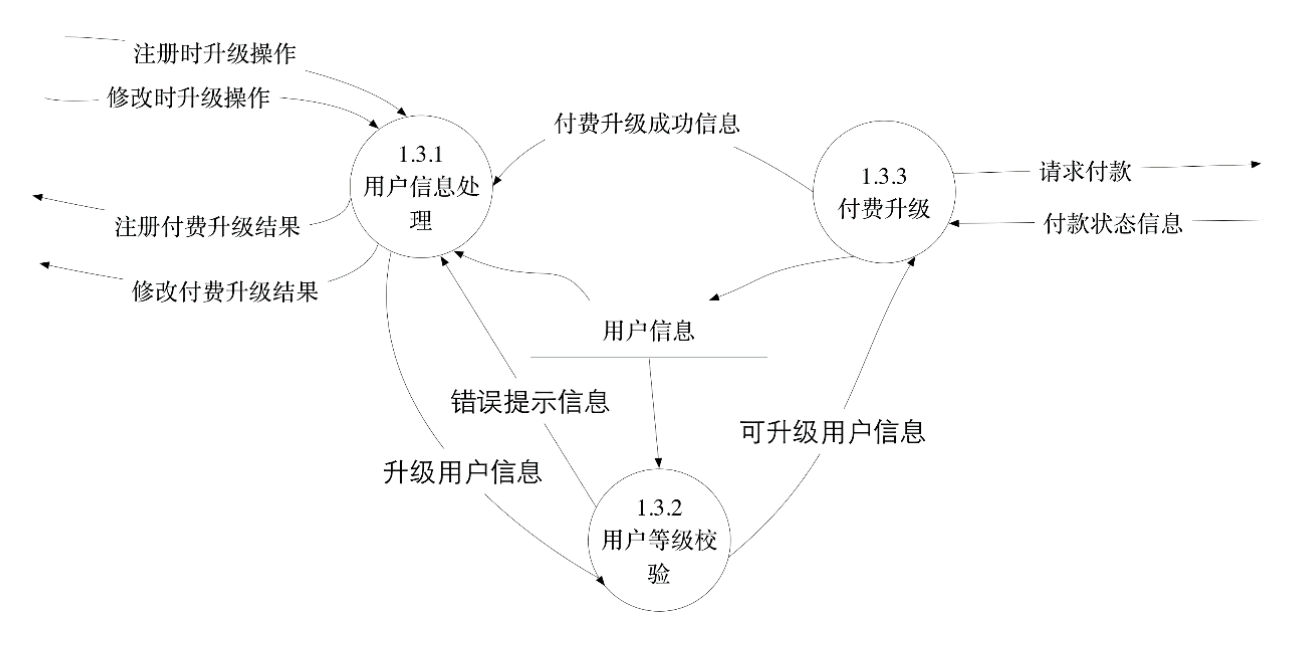
\includegraphics{img/1.3.png}
\subsubsection{浏览导航}
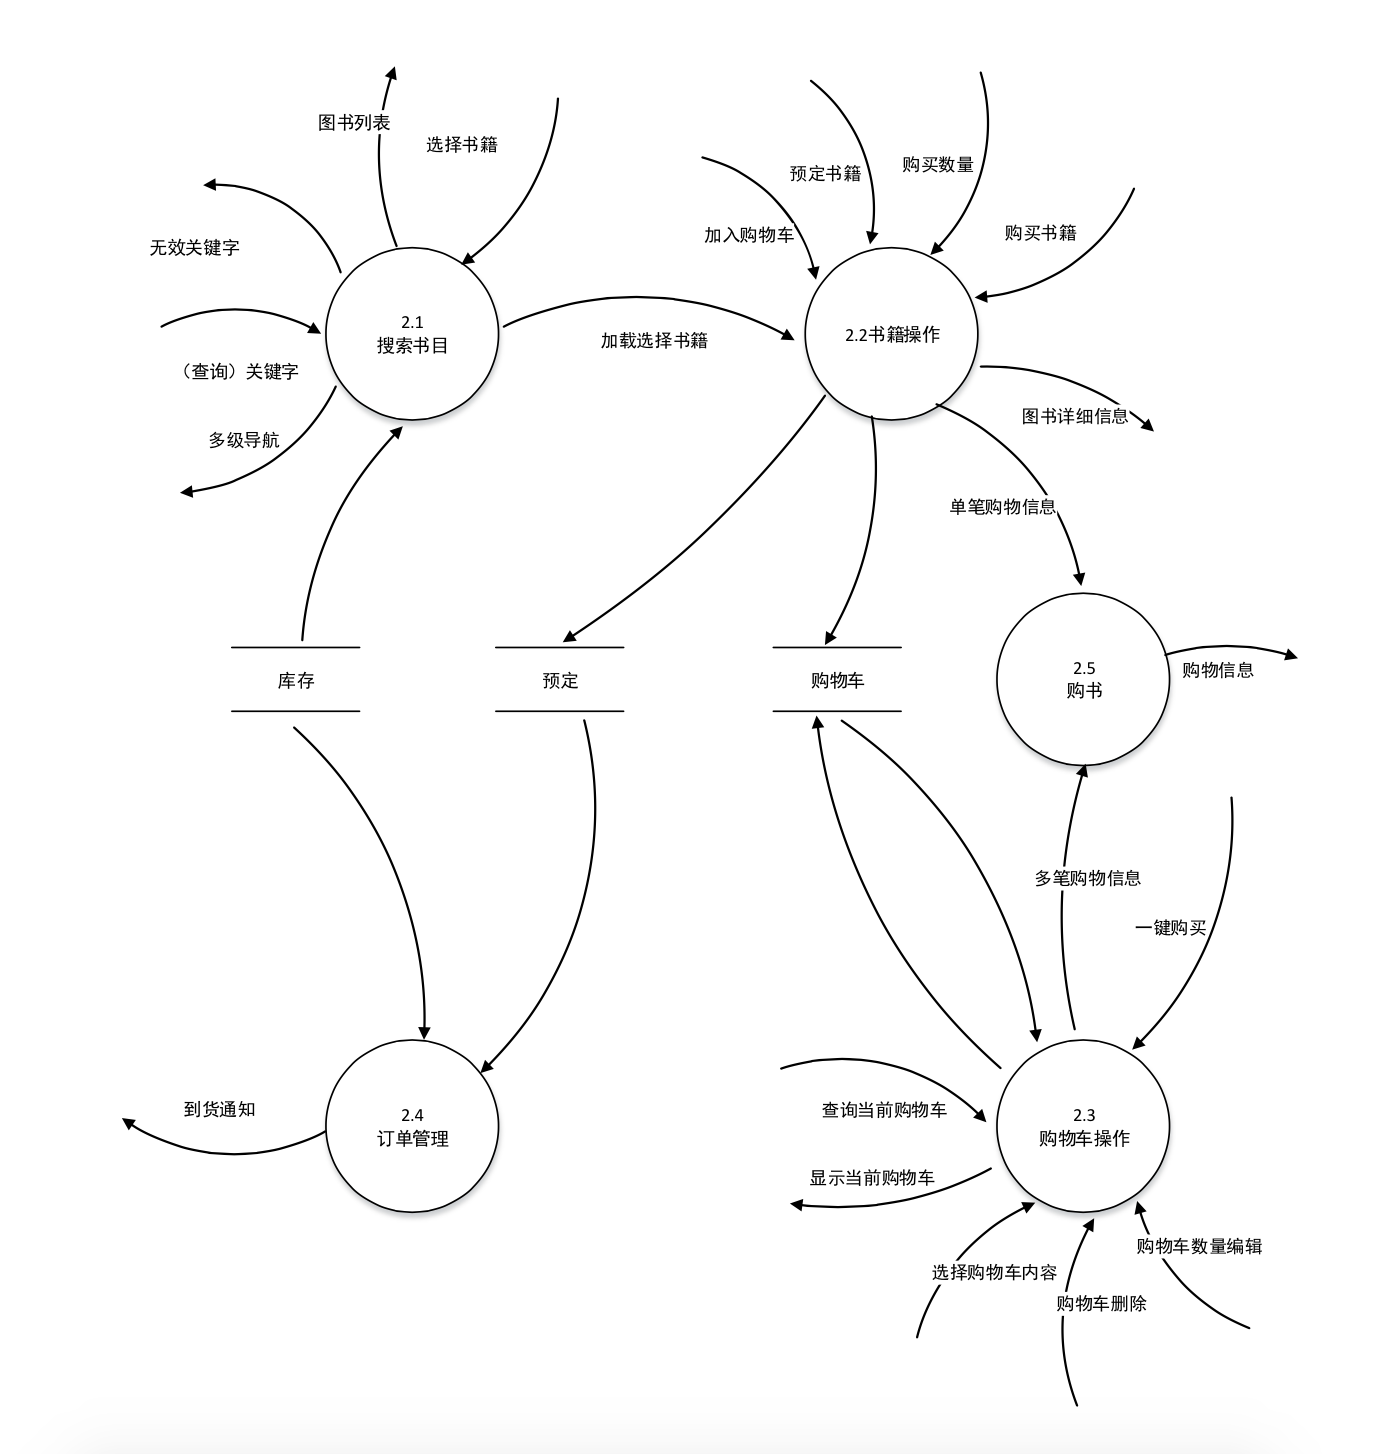
\includegraphics{img/2.png}
\paragraph{搜索书目}
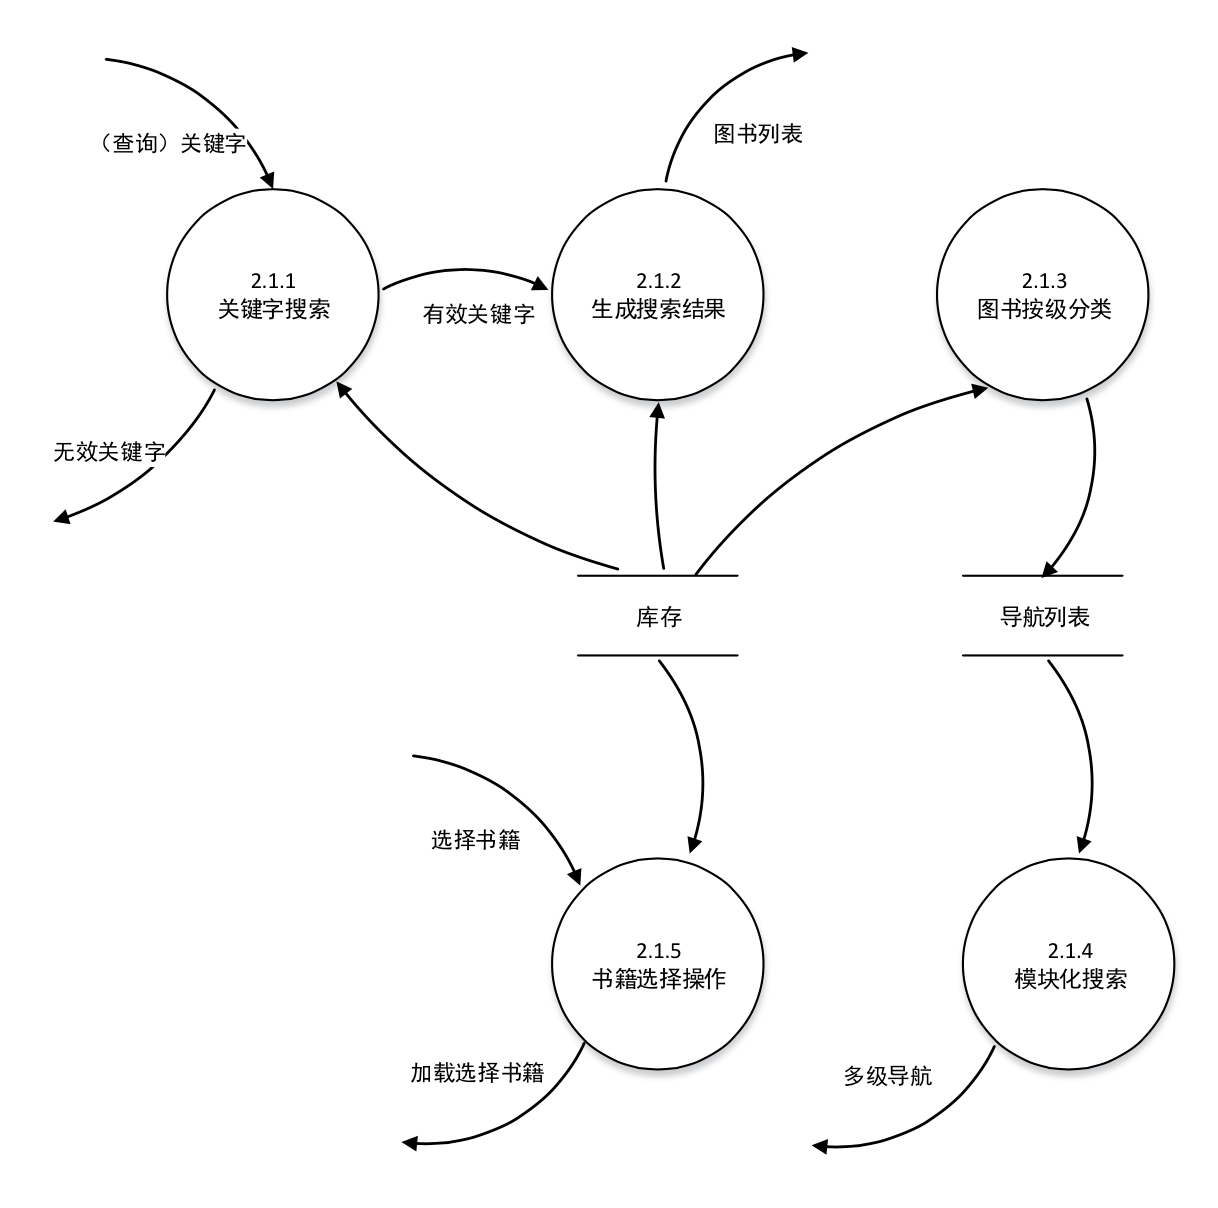
\includegraphics{img/2.1.png}
\paragraph{书籍操作}
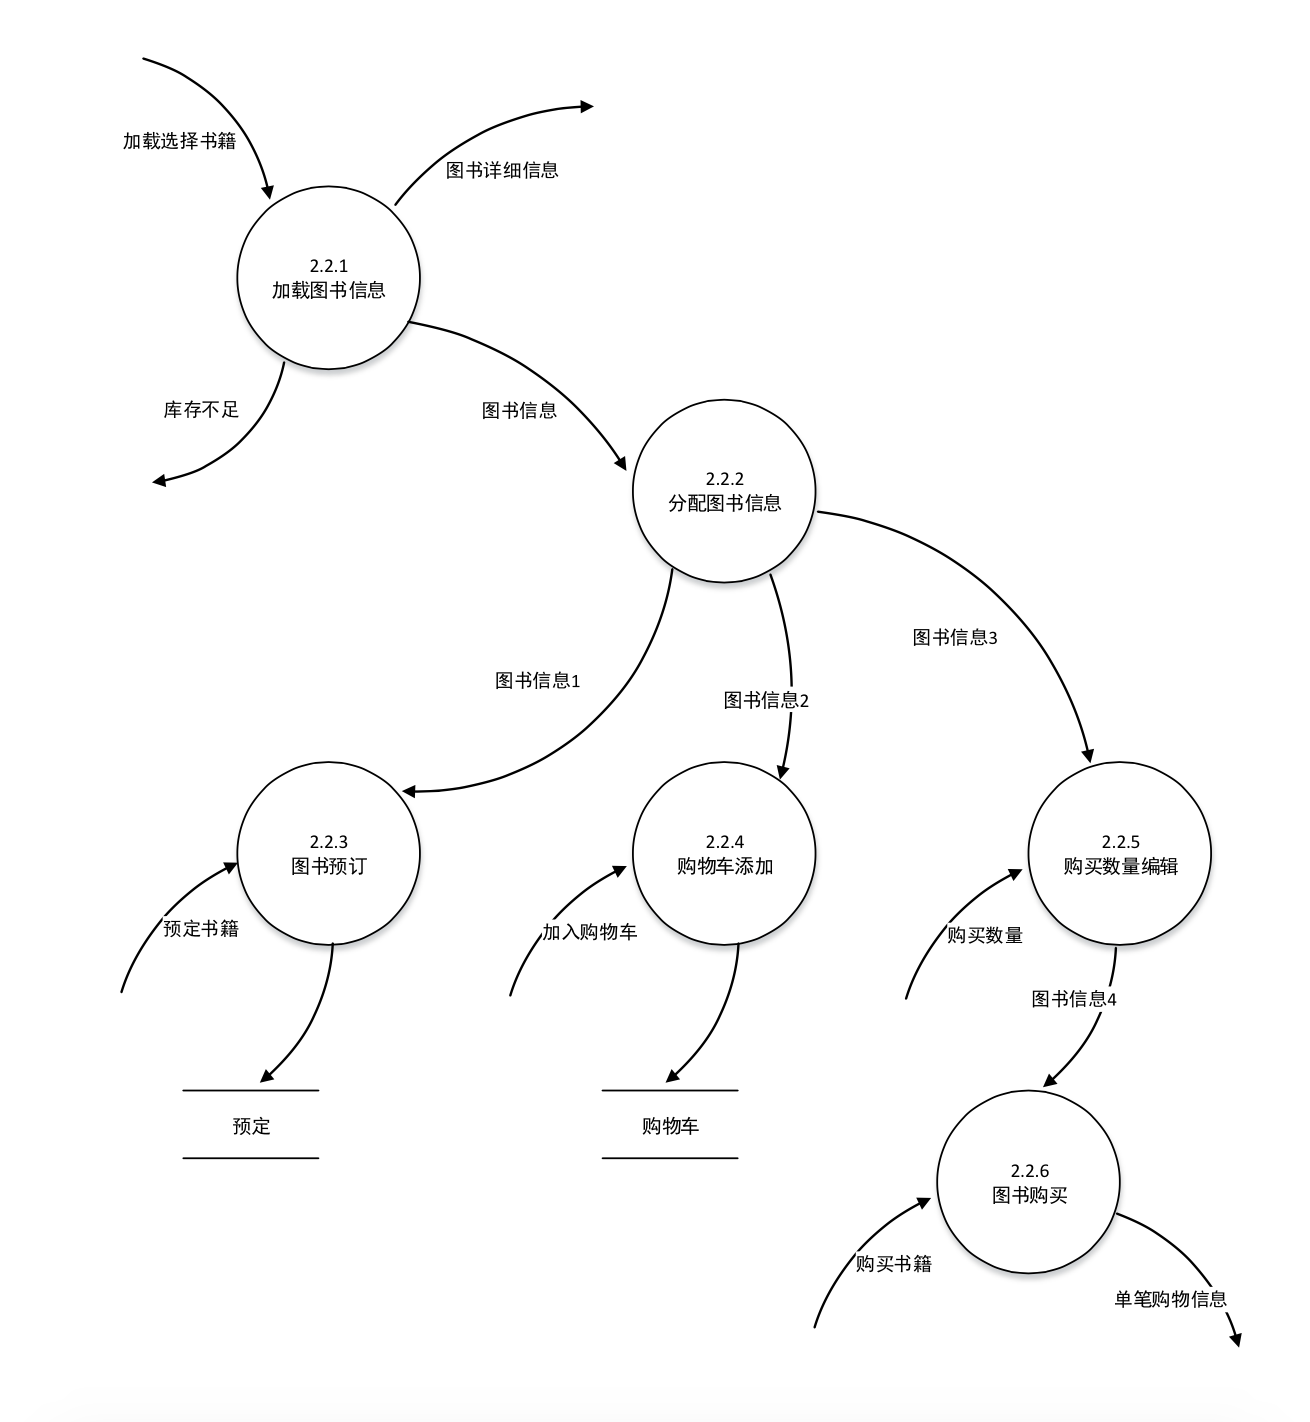
\includegraphics{img/2.2.png}
\paragraph{购物车操作}
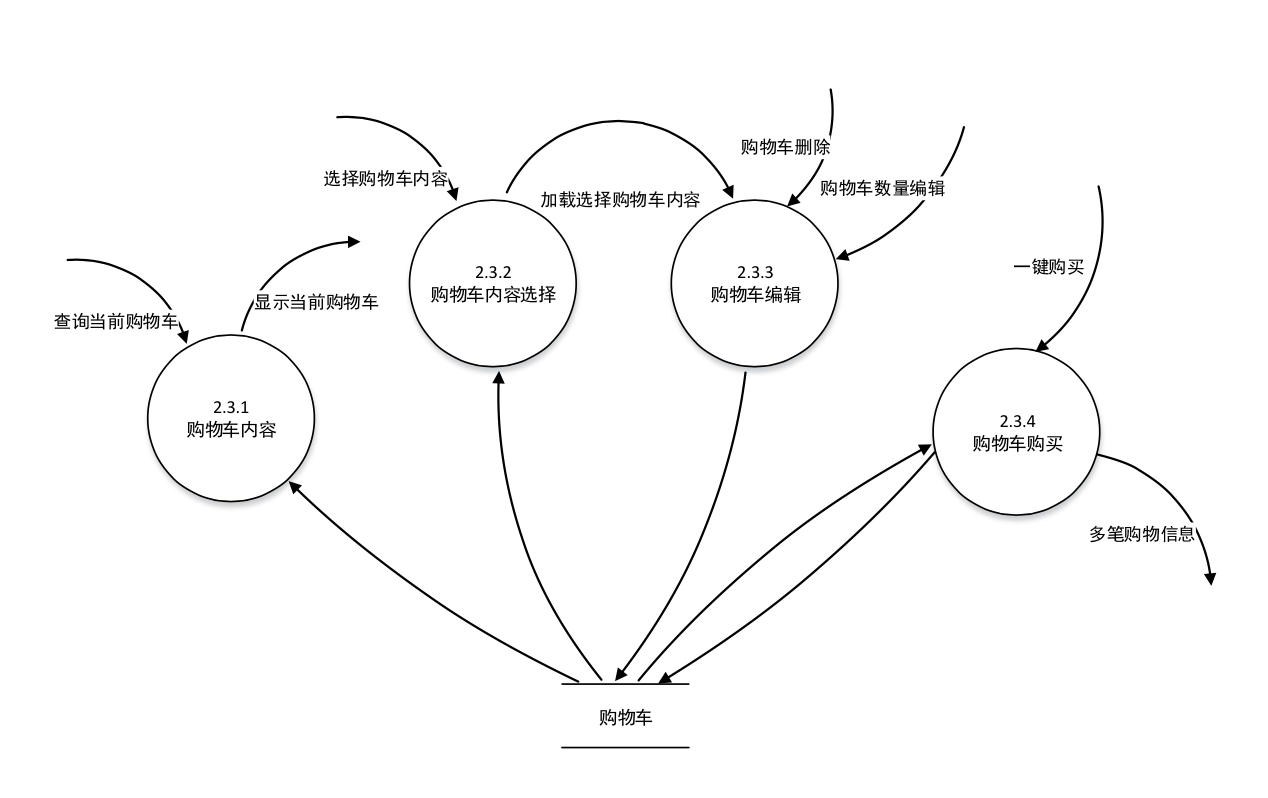
\includegraphics{img/2.3.png}
\subsubsection{订单系统}
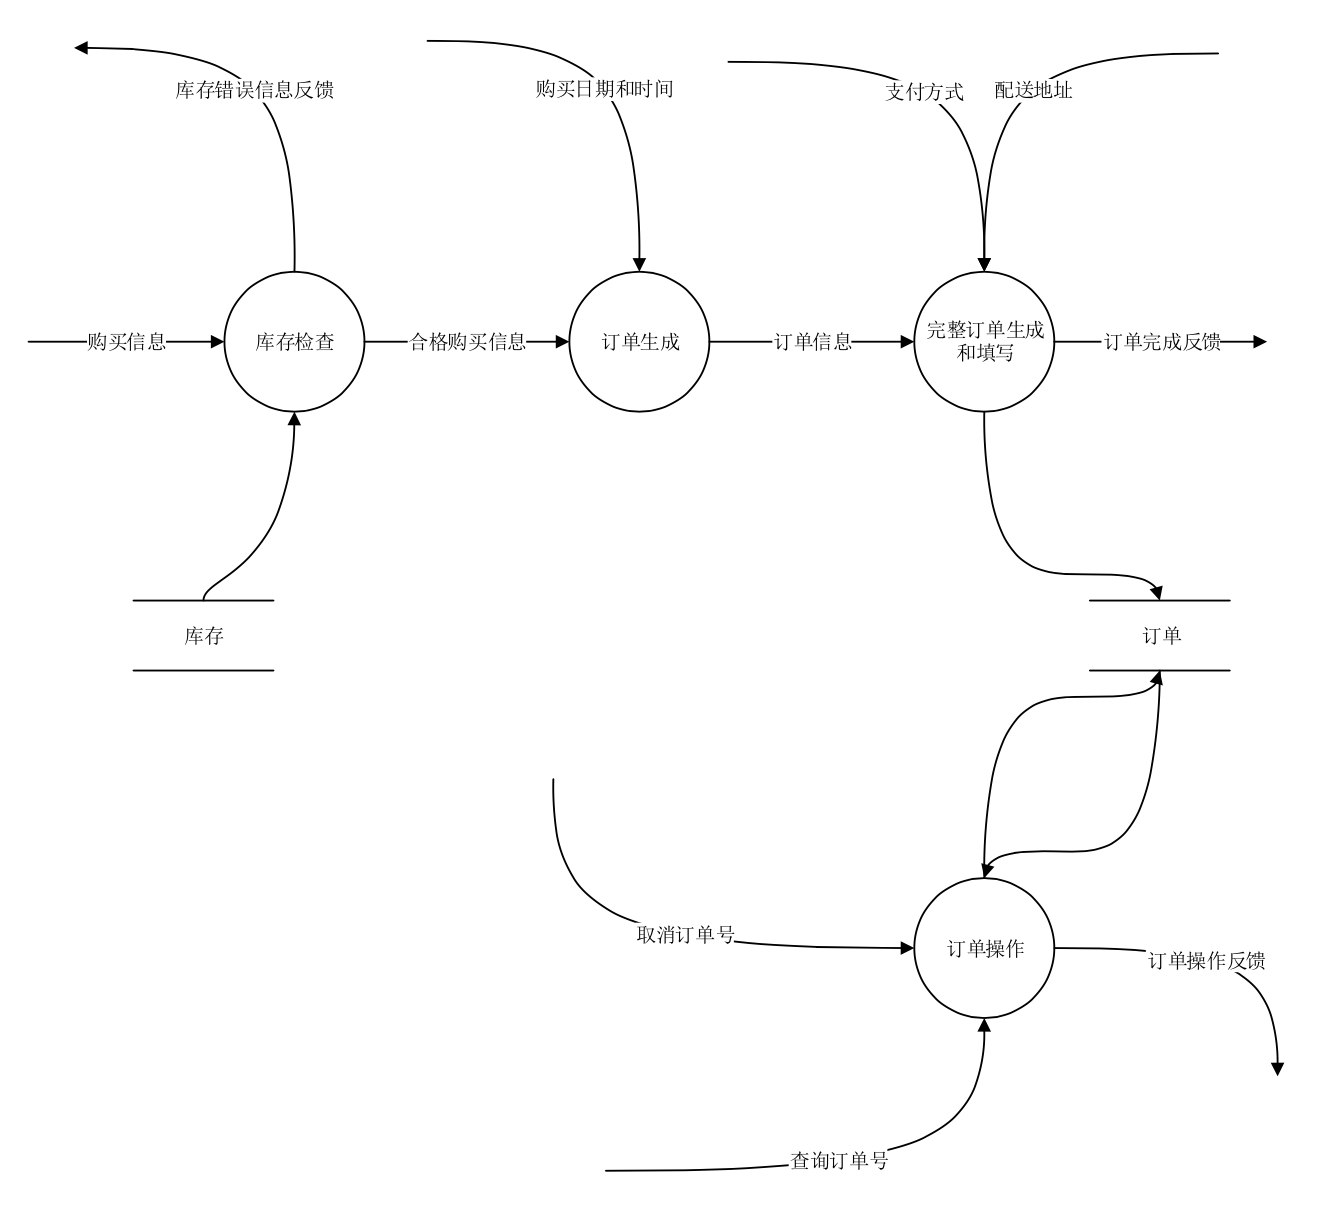
\includegraphics{img/3.png}
\paragraph{订单生成}
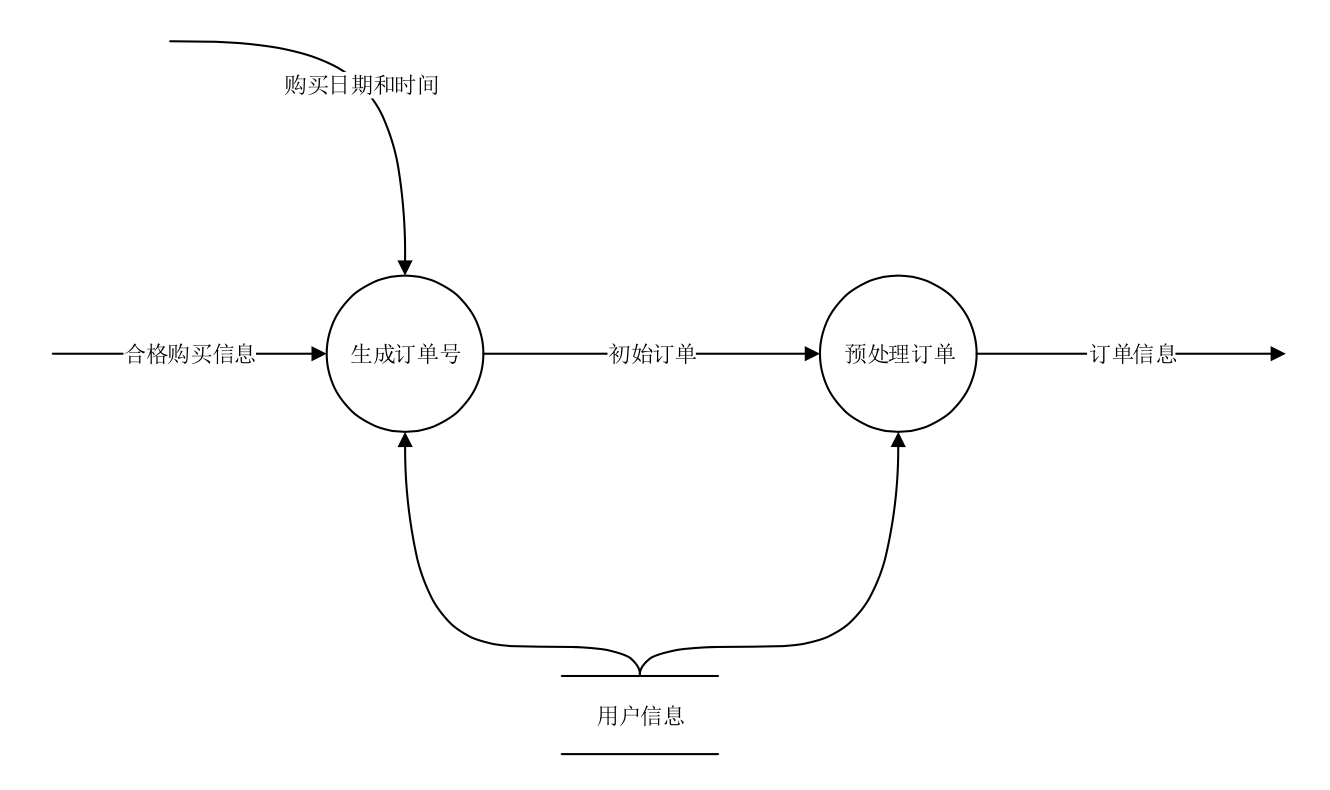
\includegraphics{img/3.2.png}
\paragraph{订单填写}
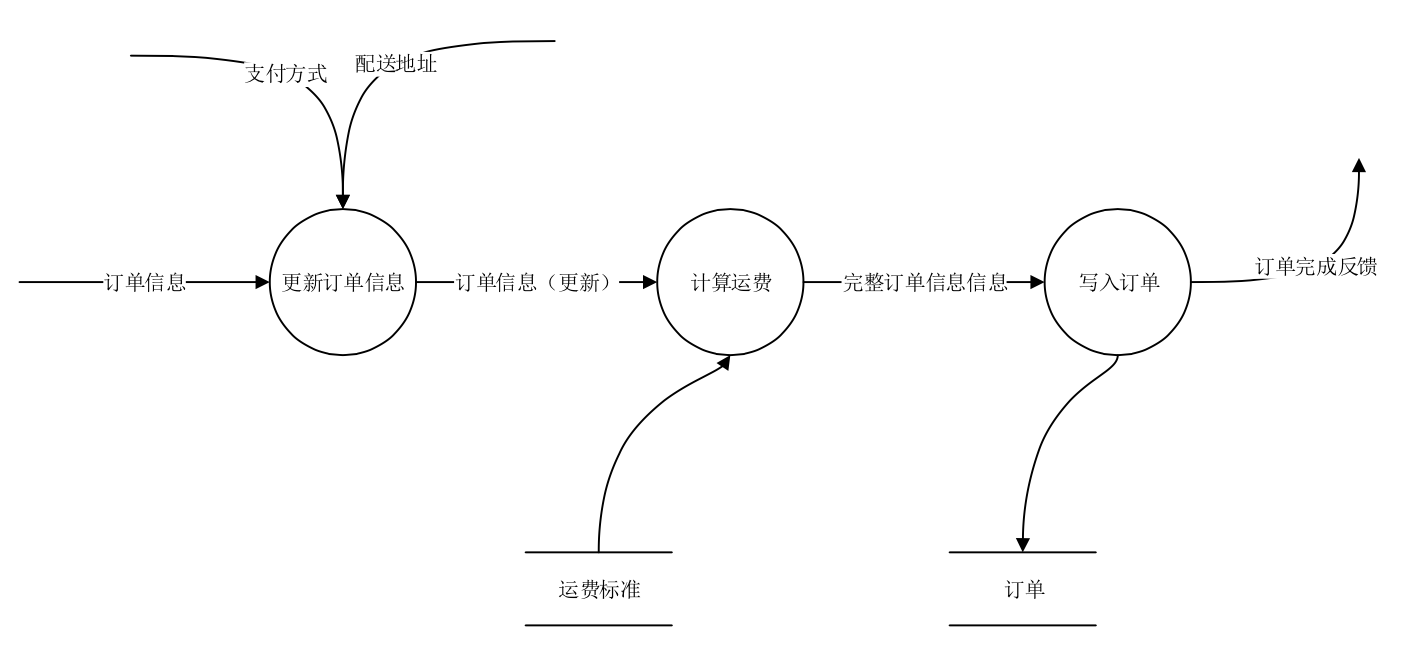
\includegraphics{img/3.3.png}
\paragraph{订单操作}
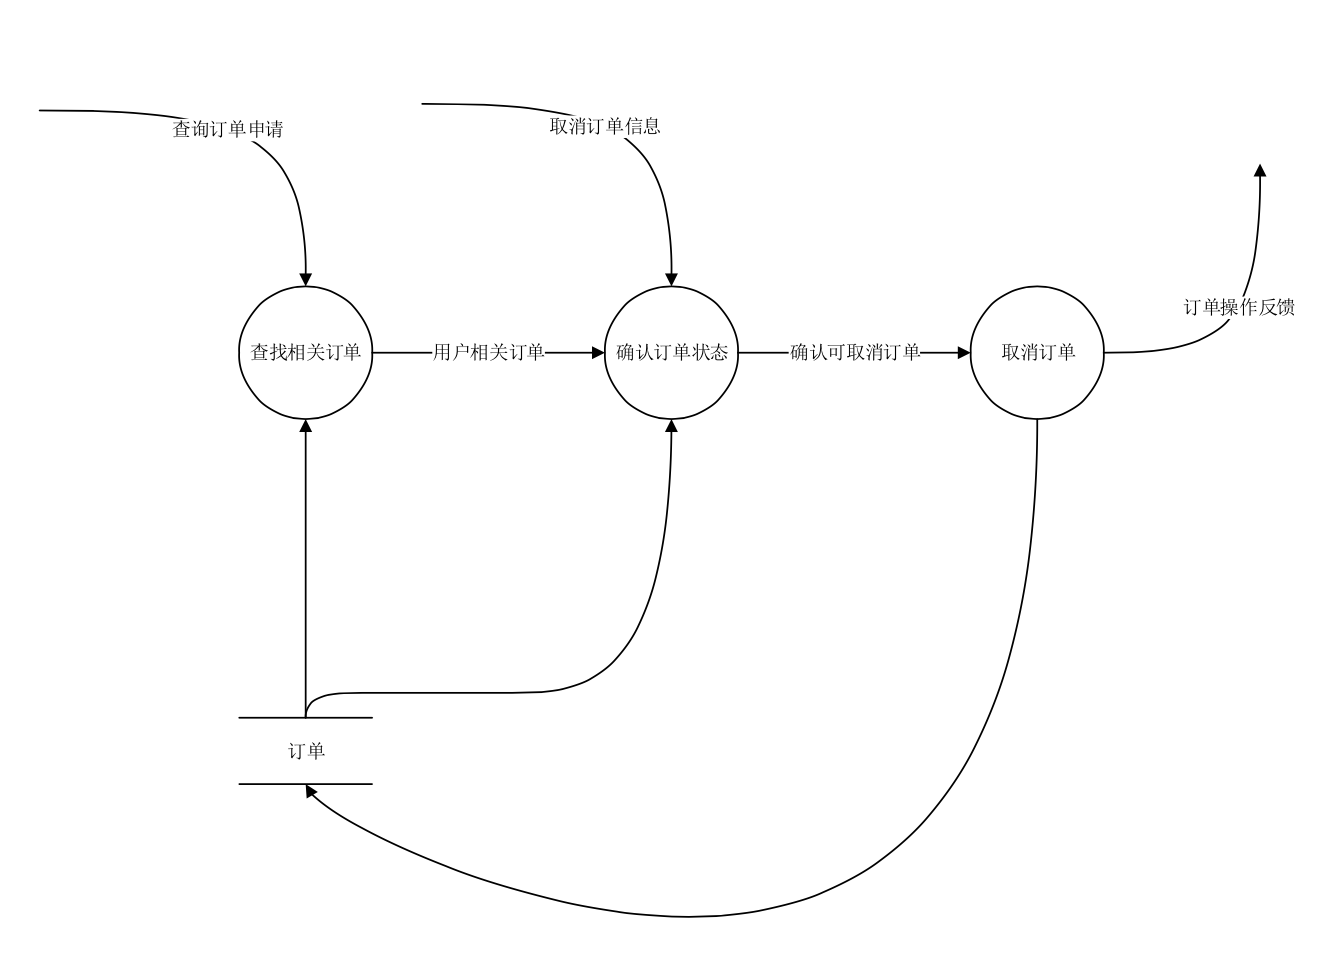
\includegraphics{img/3.4.png}
\subsubsection{支付系统}
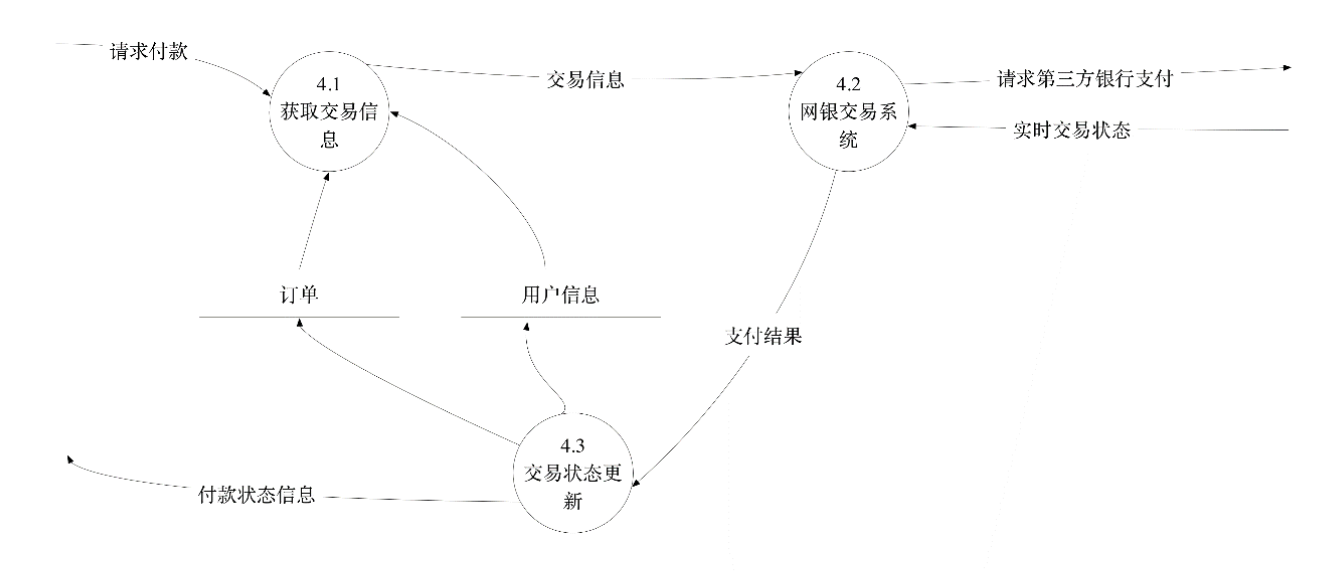
\includegraphics{img/4.png}
\subsubsection{物流管理}
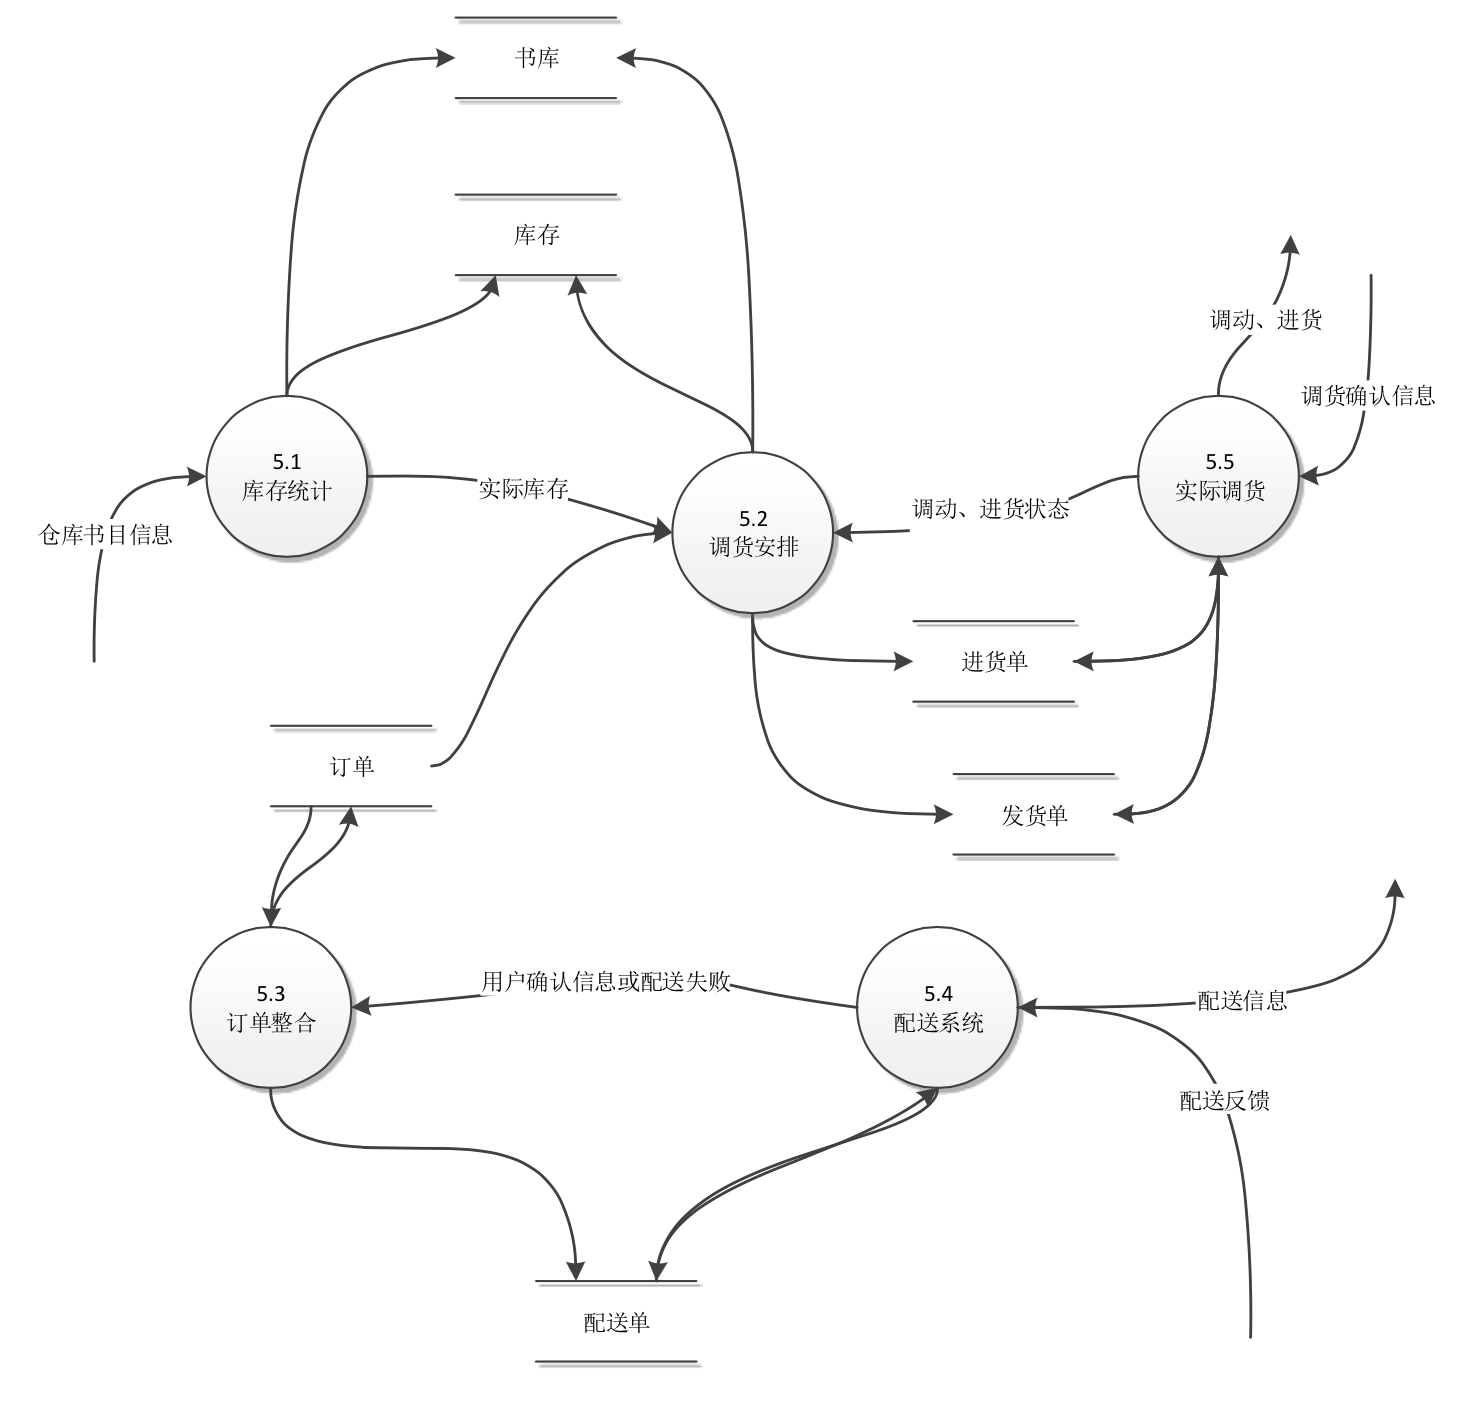
\includegraphics{img/5.png}
\paragraph{库存统计}
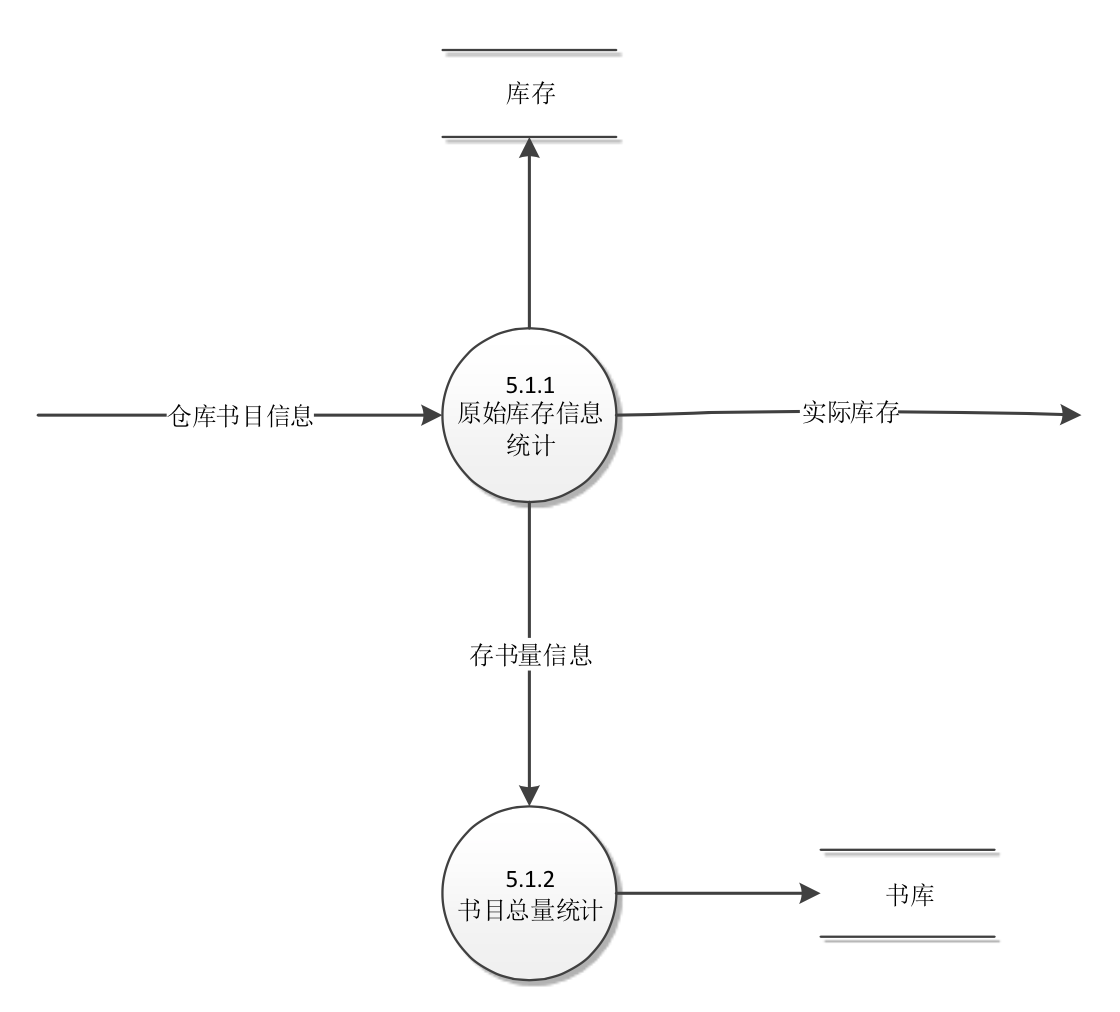
\includegraphics{img/5.1.png}
\paragraph{调货安排}
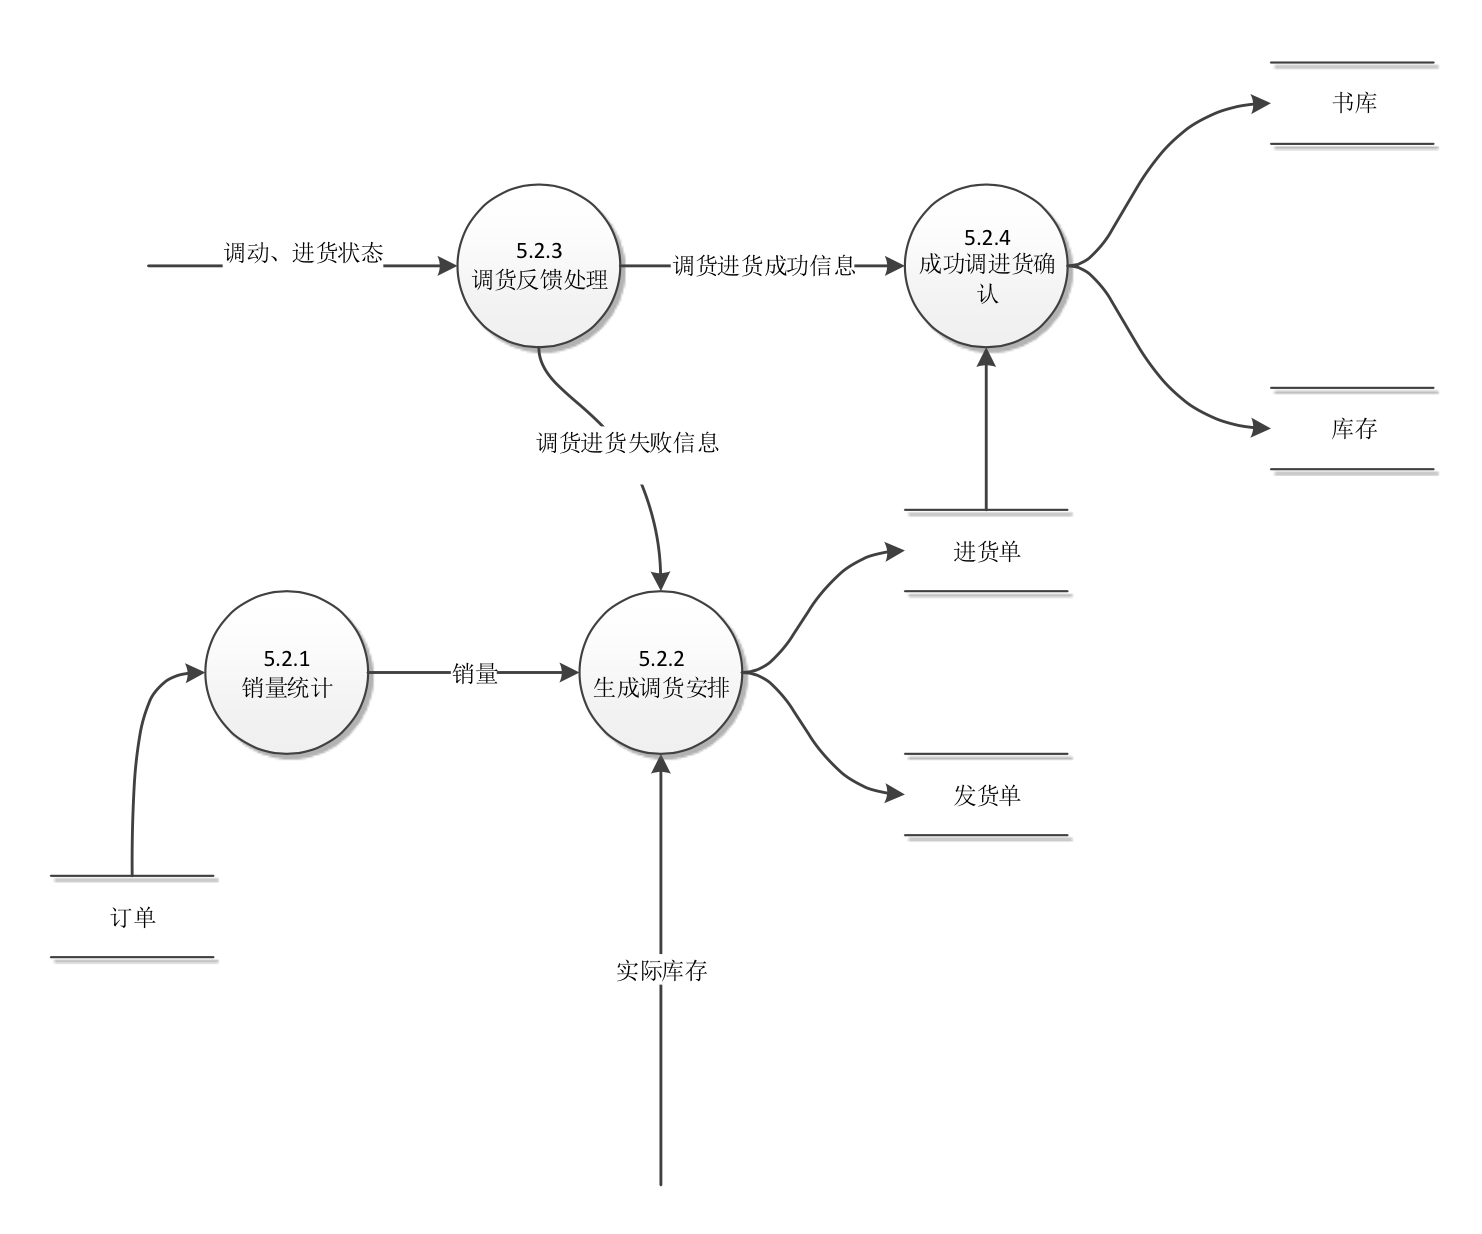
\includegraphics{img/5.2.png}
\paragraph{订单整合}
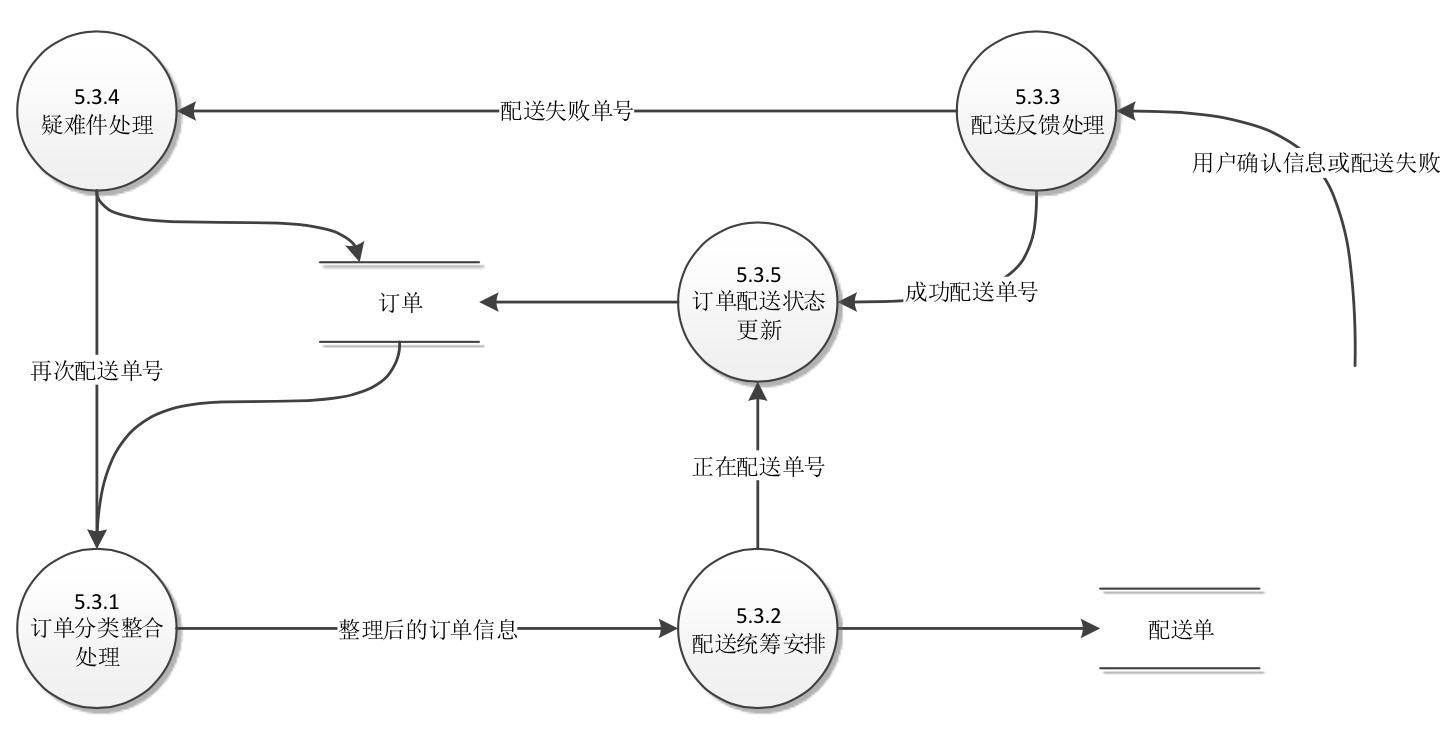
\includegraphics{img/5.3.png}
\paragraph{配送系统}
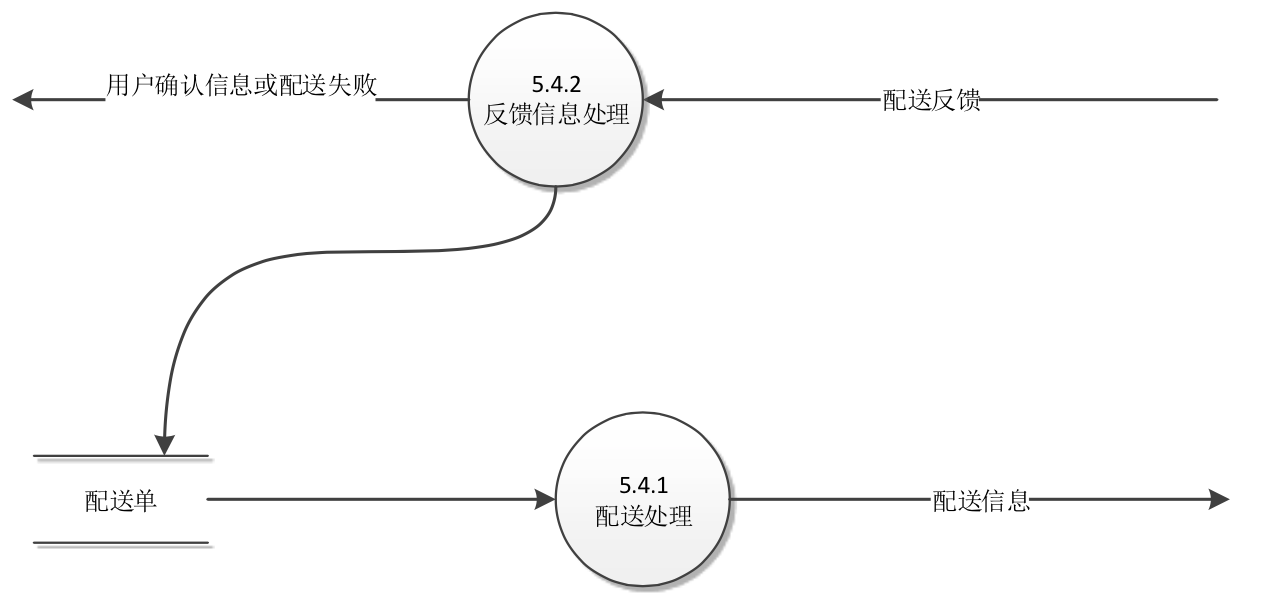
\includegraphics{img/5.4.png}
\paragraph{实际调货}
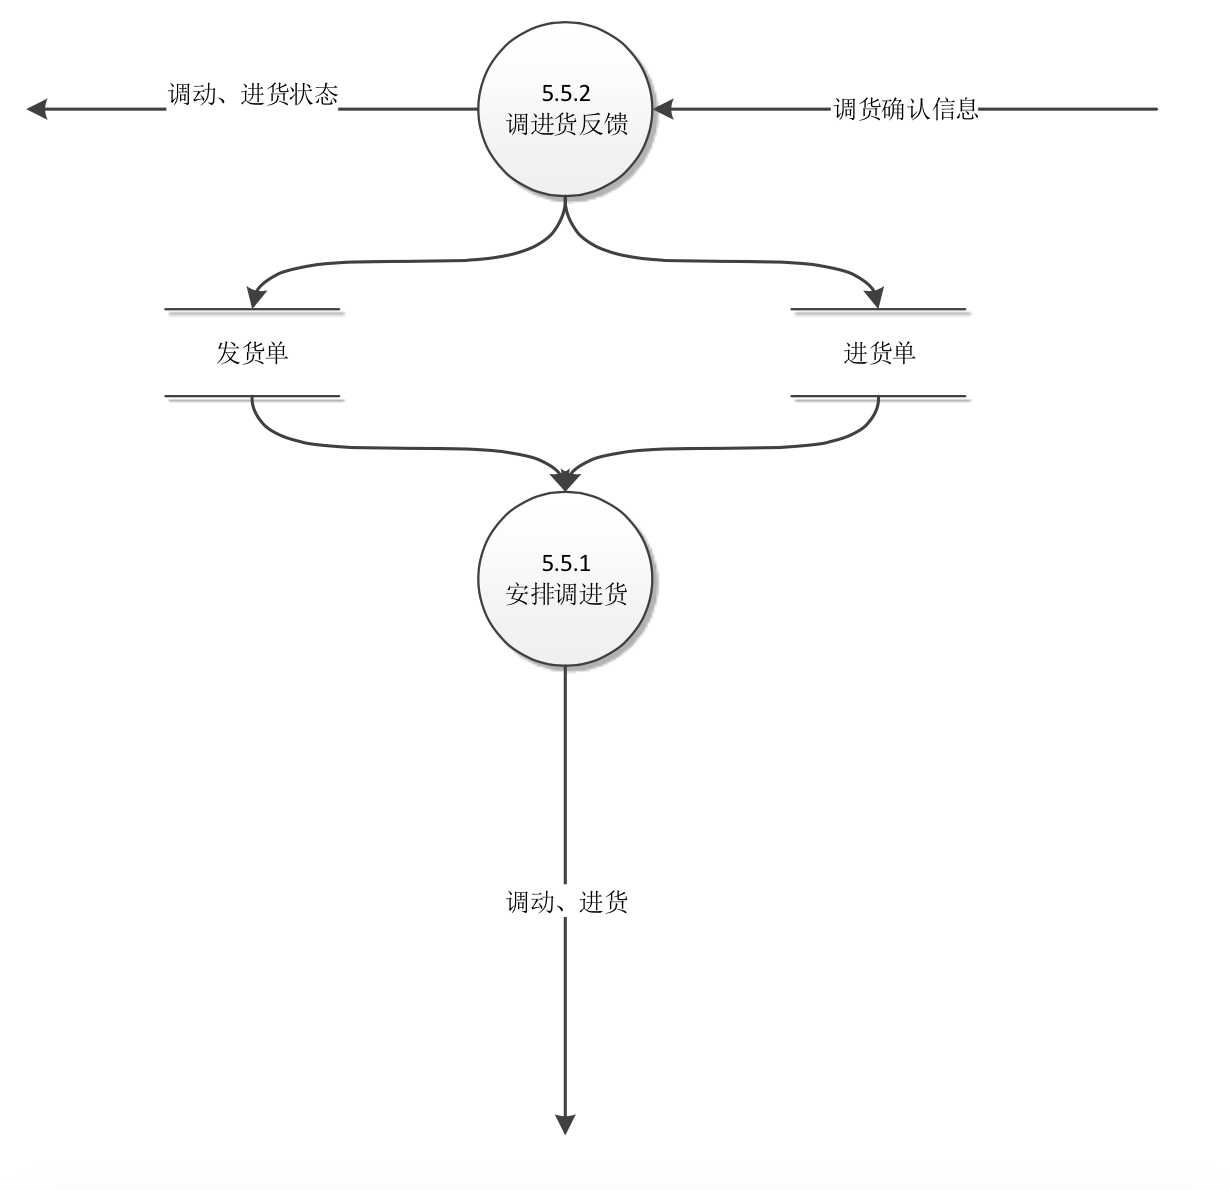
\includegraphics{img/5.5.png}
\section{数据字典}
\subsection{数据流条目}

\begin{itemize}
	\item \textit{名称:}(查询)关键字
	\item \textit{简述:}用户通过关键字搜索时在搜索框中输入的检索关键字
	\item \textit{数据流组成:}(查询)关键字 = [字符|空格符]
	\item \textit{数据流来源:}用户
	\item \textit{数据流去向:}加工 2.1.1 关键字搜索
	\item \textit{注解:}关键字之间以一个或多个空格分隔,一次可输入一个或多个关键字,但至少要输入一个关键字才能进行搜索
\end{itemize}

\vspace{-1mm}

\begin{itemize}
	\item \textit{名称:}无效关键字
	\item \textit{简述:}用户输入的关键字未能搜索到对应书目时的返回信息
	\item \textit{数据流组成:}无效关键字 = (查询)关键字 + 搜索失败提示语
	\item \textit{数据流来源:}加工 2.1.1 关键字搜索
	\item \textit{数据流去向:}用户
	\item \textit{注解:}对于搜索的书目不存在的以及输入格式不符合要求的,都返回这条消息
\end{itemize}

\vspace{-1mm}

\begin{itemize}
	\item \textit{名称:}有效关键字
	\item \textit{简述:}用户输入的关键字搜索到对应书目时系统内部的传递信息
	\item \textit{数据流组成:}有效关键字 = (查询)关键字
	\item \textit{数据流来源:}加工 2.1.1 关键字搜索
	\item \textit{数据流去向:}加工 2.1.2 生成搜索结果
	\item \textit{注解:}对于文件库存中存有的,但是目前库存数量为 0 的书目进行搜索,也返回这个结果
\end{itemize}

\vspace{-1mm}

\begin{itemize}
	\item \textit{名称:}图书列表
	\item \textit{简述:}根据用户输入的有效关键字进行搜索产生的书目列表
	\item \textit{数据流组成:}图书列表元素 = 书名 + isbn + 作者 + 出版社 + 价格
	\item \textit{数据流来源:}加工 2.1.2 生成搜索结果
	\item \textit{数据流去向:}用户
\end{itemize}

\vspace{-1mm}

\begin{itemize}
	\item \textit{名称:}多级导航
	\item \textit{简述:}通过多级分类的形式,让用户能快速搜寻到自己感兴趣的类型的书目
	\item \textit{数据流组成:}多级导航 = [一级主题类型|二级主题类型|三级主题类型]
	\item \textit{数据流来源:}2.1.4 模块化搜索
	\item \textit{数据流去向:}用户
	\item \textit{注解:}一级主题类型可细分为多个二级主题类型,这些二级主题类型都包含于该一级主题类型。同理三级主题类型都包含于某二级主题中
\end{itemize}

\vspace{-1mm}

\begin{itemize}
	\item \textit{名称:}选择书籍
	\item \textit{简述:}用户通过点击操作,选择并进入某特定书籍的操作界面
	\item \textit{数据流组成:}选择书籍 = [是|否]
	\item \textit{数据流来源:}用户
	\item \textit{数据流去向:}加工 2.1.5 书籍选择操作
\end{itemize}

\vspace{-1mm}

\begin{itemize}
	\item \textit{名称:}加载选择书籍
	\item \textit{简述:}用户点击选择了特定书籍后,系统从库存文件中读出的该图书的全部信息
	\item \textit{数据流组成:}加载选择书籍 = 书名 + isbn + 作者 + 出版社 + 价格 + 存量
	\item \textit{数据流来源:}加工 2.1.5 书籍选择操作
	\item \textit{数据流去向:}加工 2.2.1 加载图书信息
\end{itemize}

\vspace{-1mm}

\begin{itemize}
	\item \textit{名称:}库存不足
	\item \textit{简述:}当用户选择的书籍没有库存时,提示用户进行预定
	\item \textit{数据流组成:}库存不足 = 书名 + isbn + 库存不足提示 + 预定提示
	\item \textit{数据流来源:}加工 2.2.1 加载图书信息
	\item \textit{数据流去向:}用户
\end{itemize}

\vspace{-1mm}

\begin{itemize}
	\item \textit{名称:}图书详细信息
	\item \textit{简述:}将系统从库存文件中读出的图书信息显示给用户
	\item \textit{数据流组成:}图书详细信息 = 加载选择书籍
	\item \textit{数据流来源:}加工 2.2.1 加载图书信息
	\item \textit{数据流去向:}用户
\end{itemize}

\vspace{-1mm}

\begin{itemize}
	\item \textit{名称:}图书信息
	\item \textit{简述:}系统内部传递与分配所需的图书的全部信息
	\item \textit{数据流组成:}图书详细信息 = 加载选择书籍
	\item \textit{数据流来源:}加工 2.2.1 加载图书信息
	\item \textit{数据流去向:}加工 2.2.2 分配图书信息
\end{itemize}

\vspace{-1mm}

\begin{itemize}
	\item \textit{名称:}预定书籍
	\item \textit{简述:}用户选择特定书籍进行预定操作的信号
	\item \textit{数据流组成:}预定书籍 = [是|否]
	\item \textit{数据流来源:}用户
	\item \textit{数据流去向:}加工 2.2.3 图书预定
	\item \textit{注解:}只有当前库存为零的书籍才能进行预定操作
\end{itemize}

\vspace{-1mm}

\begin{itemize}
	\item \textit{名称:}购物车图书信息
	\item \textit{简述:}提供添加购物车所需的图书信息
	\item \textit{数据流组成:}购物车图书信息  = 书名 + isbn + 价格
	\item \textit{数据流来源:}加工 2.2.2 分配图书信息
	\item \textit{数据流去向:}加工 2.2.4 购物车添加
\end{itemize}

\vspace{-1mm}

\begin{itemize}
	\item \textit{名称:}加入购物车
	\item \textit{简述:}用户选择特定书籍加入购物车的信号
	\item \textit{数据流组成:}加入购物车 = [是|否]
	\item \textit{数据流来源:}用户
	\item \textit{数据流去向:}加工 2.2.4 购物车添加
	\item \textit{注解:}加入购物车的图书数量都默认为 1。若要一次购买多本,可在加工 2.3 购物车操作中	进行数量编辑
\end{itemize}

\vspace{-1mm}

\begin{itemize}
\item \textit{名称:}预购图书信息
\item \textit{简述:}提供购买操作所需的图书信息
\item \textit{数据流组成:}预购图书信息  = 书名 + isbn + 价格
\item \textit{数据流来源:}加工 2.2.2 分配图书信息
\item \textit{数据流去向:}加工 2.2.5 购买数量编辑
\end{itemize}

\vspace{-1mm}

\begin{itemize}
	\item \textit{名称:}购买数量
	\item \textit{简述:}用户输入的选择图书的购买数量
	\item \textit{数据流组成:}购买数量 = 非负整数值
	\item \textit{数据流来源:}用户
	\item \textit{数据流去向:}加工 2.2.5 购买数量编辑
	\item \textit{注解:}用户输入的购买数量必须不小于 0,且不大于库存余量。如果用户输入的数值超出库存余量,则将其默认为库存余量。用户若想要购买更多,则需通过预定操作,并等待库存更新
\end{itemize}

\vspace{-1mm}

\begin{itemize}
	\item \textit{名称:}图书购买信息
	\item \textit{简述:}提供生成购物信息所需的图书信息,并加入了购买数量
	\item \textit{数据流组成:}图书购买信息  = 预购图书信息 + 数量
	\item \textit{数据流来源:}加工 2.2.5 购买数量编辑
	\item \textit{数据流去向:}加工 2.2.6 图书购买
\end{itemize}

\vspace{-1mm}

\begin{itemize}
	\item \textit{名称:}购买书籍
	\item \textit{简述:}用户选择特定书籍进行购买的信号
	\item \textit{数据流组成:}购买书籍 = [是|否]
	\item \textit{数据流来源:}用户
	\item \textit{数据流去向:}加工 2.2.6 图书购买
\end{itemize}

\vspace{-1mm}

\begin{itemize}
	\item \textit{名称:}单笔购物信息
	\item \textit{简述:}用户在某图书页面点击购买之后生成的购物信息
	\item \textit{数据流组成:}单笔购物信息 = 书名 + isbn +价格 + 数量
	\item \textit{数据流来源:}加工 2.2.6 图书购买
	\item \textit{数据流去向:}加工 2.5 购书
\end{itemize}

\vspace{-1mm}

\begin{itemize}
	\item \textit{名称:}查询当前购物车
	\item \textit{简述:}用户对当前购物车内容进行查询的信号
	\item \textit{数据流组成:}查询当前购物车 = [是|否]
	\item \textit{数据流来源:}用户
	\item \textit{数据流去向:}加工 2.3.1 购物车内容
\end{itemize}

\vspace{-1mm}

\begin{itemize}
	\item \textit{名称:}显示当前购物车
	\item \textit{简述:}对“查询当前购物车”的反馈,显示当前购物车内容
	\item \textit{数据流组成:}显示当前购物车 = 书名 + isbn +价格 + 数量
	\item \textit{数据流来源:}加工 2.3.1 购物车内容
	\item \textit{数据流去向:}用户
\end{itemize}

\vspace{-1mm}

\begin{itemize}
	\item \textit{名称:}选择购物车内容
	\item \textit{简述:}用户选择特定的购物车内容以进行编辑的信号
	\item \textit{数据流组成:}选择购物车内容 = [是|否]
	\item \textit{数据流来源:}用户
	\item \textit{数据流去向:}加工 2.3.2 购物车内容选择
\end{itemize}

\vspace{-1mm}

\begin{itemize}
	\item \textit{名称:}加载选择购物车内容
	\item \textit{简述:}根据用户的选择显示特定的购物车内容的详细信息,以便用户进行编辑
	\item \textit{数据流组成:}加载选择购物车内容 = 书名 + isbn + 价格 + 数量
	\item \textit{数据流来源:}加工 2.3.2 购物车内容选择
	\item \textit{数据流去向:}加工 2.3.3 购物车编辑
\end{itemize}

\vspace{-1mm}

\begin{itemize}
	\item \textit{名称:}购物车数量编辑
	\item \textit{简述:}用户对选中的特定购物车内容进行更改数量的操作
	\item \textit{数据流组成:}购物车数量编辑 = 大于 0 的整数
	\item \textit{数据流来源:}用户
	\item \textit{数据流去向:}加工 2.3.3 购物车编辑
\end{itemize}

\vspace{-1mm}

\begin{itemize}
	\item \textit{名称:}购物车删除
	\item \textit{简述:}用户删除选中的特定购物车内容的操作
	\item \textit{数据流组成:}购物车删除 = [是|否]
	\item \textit{数据流来源:}用户
	\item \textit{数据流去向:}加工 2.3.3 购物车编辑
\end{itemize}

\vspace{-1mm}

\begin{itemize}
	\item \textit{名称:}一键购买
	\item \textit{简述:}用户通过购物车,对购物车内的图书进行一次性购买的操作信号
	\item \textit{数据流组成:}一键购买 = [是|否]
	\item \textit{数据流来源:}用户
	\item \textit{数据流去向:}加工 2.3.4 购物车购买
	\item \textit{注解:}该操作仅在购物车不为空时有效
\end{itemize}

\vspace{-1mm}

\begin{itemize}
	\item \textit{名称:}多笔购物信息
	\item \textit{简述:}用户通过购物车一键购买后生成的购物信息
	\item \textit{数据流组成:}多笔购物信息 = 
	\item \textit{数据流来源:}加工 2.3.4 购物车购买
	\item \textit{数据流去向:}加工 2.5 购买
\end{itemize}

\vspace{-1mm}

\begin{itemize}
	\item \textit{名称:}到货通知
	\item \textit{简述:}用户预定的图书到货后,向用户发送的通知
	\item \textit{数据流组成:}到货通知 = 书名 + 到货提示信息
	\item \textit{数据流来源:}加工 2.4 预定管理
	\item \textit{数据流去向:}用户
\end{itemize}

\vspace{-1mm}

\begin{itemize}
	\item \textit{名称:}购物信息
	\item \textit{简述:}整合后的所有购物信息,用以生成订单
	\item \textit{数据流组成:}购物信息 =
	\item \textit{数据流来源:}加工 2.5 购物信息
	\item \textit{数据流去向:}加工 3 订单系统
\end{itemize}

\vspace{-1mm}

\begin{itemize}
	\item \textit{名称:}购买信息
	\item \textit{简述:}由浏览导航子系统发出的用户购买信息,用于生成订单
	\item \textit{数据流组成:}购买信息=商品ID+商品名称+商品单价+购买数量+用户I
	\item \textit{数据流来源:}浏览导航
	\item \textit{数据流去向:}加工3.1 库存检查
	\item \textit{注解:}购买信息由购物车生成,相当于用户提交的一个购物申请
\end{itemize}

\vspace{-1mm}

\begin{itemize}
	\item \textit{名称:}库存错误反馈
	\item \textit{简述:}对购买信息进行库存检查后,返回的错误反馈
	\item \textit{数据流组成:}库存错误反馈=商品ID+商品名称+购买数量+用户ID
	\item \textit{数据流来源:}加工3.1 库存检查
	\item \textit{数据流去向:}浏览导航
	\item \textit{注解:}由于很可能单次购买中的货品仍有库存,但不能满足此次购买的数量,因此反馈数据流中仍需要注明购买数量,而不仅仅是反馈没有库存的货品
\end{itemize}

\vspace{-1mm}

\begin{itemize}
	\item \textit{名称:}合格购买信息
	\item \textit{简述:}通过库存检查后,确认有货的购买信息
	\item \textit{数据流组成:}合格信息=商品ID+商品名称+商品单价+购买数量+用户ID
	\item \textit{数据流来源:}加工3.1 库存检查
	\item \textit{数据流去向:}加工3.2.1 生成订单号
\end{itemize}

\vspace{-1mm}

\begin{itemize}
	\item \textit{名称:}购买日期和时间
	\item \textit{简述:}获取此次购买的日期和时间,用户生成唯一的订单号
	\item \textit{数据流组成:}购买日期和时间=购买日期+购买时间
	\item \textit{数据流来源:}服务器生成
	\item \textit{数据流去向:}加工3.2.1 生成订单号
\end{itemize}

\vspace{-1mm}

\begin{itemize}
	\item \textit{名称:}初始订单
	\item \textit{简述:}对单个购买信息生成并分配的唯一订单号,保证后续操作
	\item \textit{数据流组成:}初始订单=商品ID+商品名称+商品单价+购买数量+用户ID+订单号
	\item \textit{数据流来源:}加工3.2.1 生成订单号
	\item \textit{数据流去向:}加工3.2.2 预处理订单
\end{itemize}

\vspace{-1mm}

\begin{itemize}
	\item \textit{名称:}订单信息
	\item \textit{简述:}系统自动匹配用户后,向初始订单填写默认的付款方式和收货地址,形成完整的订单信息
	\item \textit{数据流组成:}订单信息=商品ID+商品名称+商品单价+购买数量+用户ID+用户名+付款方式+收货地址
	\item \textit{数据流来源:}加工3.2.2 预处理订单
	\item \textit{数据流去向:}加工3.3.1 更新订单信息
	\item \textit{注解:}初步填写一个完整的订单,方便用户操作,无需填写默认的支付方式和收货地址
\end{itemize}

\vspace{-1mm}

\begin{itemize}
	\item \textit{名称:}支付方式
	\item \textit{简述:}用户可以选择的支付方式
	\item \textit{数据流组成:}支付方式=支付方式
	\item \textit{数据流来源:}用户
	\item \textit{数据流去向:}加工3.3.1 更新订单信息
	\item \textit{注解:}用户可以选择除默认支付方式外的其他支付方式
\end{itemize}

\vspace{-1mm}

\begin{itemize}
	\item \textit{名称:}配送地址
	\item \textit{简述:}用户填写的配送地址
	\item \textit{数据流组成:}配送地址=收货地址+邮编
	\item \textit{数据流来源:}用户
	\item \textit{数据流去向:}加工3.3.1 更新订单信息
	\item \textit{注解:}用户可以选择重新填写的配送地址
\end{itemize}

\vspace{-1mm}

\begin{itemize}
	\item \textit{名称:}订单信息(更新)
	\item \textit{简述:}更新并确认支付方式和配送地址后的订单信息
	\item \textit{数据流组成:}订单信息(更新)=商品ID+商品名称+商品单价+购买数量+用户ID+用户名+付款方式+收货地址
	\item \textit{数据流来源:}加工3.3.1 更新订单信息
	\item \textit{数据流去向:}加工3.3.2 计算运费
\end{itemize}

\vspace{-1mm}

\begin{itemize}
	\item \textit{名称:}最终订单信息
	\item \textit{简述:}更新并确认支付方式和配送地址后,由货物总价加上运费价格后的订单信息,并包含初始化的订单状态
	\item \textit{数据流组成:}最终订单信息=商品ID+商品名称+商品单价+购买数量+用户ID+用户名+付款方式+收货地址+订单总价+订单状态
	\item \textit{数据流来源:}加工3.3.3 写入交易信息
	\item \textit{数据流去向:}用户
\end{itemize}

\vspace{-1mm}

\begin{itemize}
	\item \textit{名称:}查询订单申请
	\item \textit{简述:}用户提交的查询订单申请
	\item \textit{数据流组成:}查询订单号=用户ID+(查询订单号)
	\item \textit{数据流来源:}用户
	\item \textit{数据流去向:}加工 3.4.1 查找相关订单
	\item \textit{注解:}因为要确认这个订单是否为此用户生成的,因此信息中需要附带用户 ID 用于检查;可以选择特定订单号,也可以不输入订单号,罗列所有用户订单
\end{itemize}

\vspace{-1mm}

\begin{itemize}
\item \textit{名称:}用户相关订单
	\item \textit{简述:}用户提交的查询订单申请
	\item \textit{数据流组成:}查询订单号=用户ID+用户相关订单
	\item \textit{数据流来源:}用户
	\item \textit{数据流去向:}加工 3.4.2 确认订单状态
	\item \textit{注解:}发送至确认订单状态是为了便于用户从中选择需要取消的订单。
\end{itemize}

\vspace{-1mm}

\begin{itemize}
\item \textit{名称:}取消订单申请
	\item \textit{简述:}用户提交的取消订单申请
	\item \textit{数据流组成:}查询订单号=用户ID+查询订单号
	\item \textit{数据流来源:}用户
	\item \textit{数据流去向:}加工 3.4.2 确认订单状态
	\item \textit{注解:}同上。
\end{itemize}

\vspace{-1mm}

\begin{itemize}
\item \textit{名称:}确认可取消订单
	\item \textit{简述:}经过状态检查后,确认可以取消的订单
	\item \textit{数据流组成:}确认可取消订单=用户ID+取消订单号+订单状态
	\item \textit{数据流来源:}加工3.4.2 确认订单状态
	\item \textit{数据流去向:}加工 3.4.3 取消订单
\end{itemize}

\vspace{-1mm}

\begin{itemize}
\item \textit{名称:}取消订单反馈
	\item \textit{简述:}完成取消订单后的反馈信息
	\item \textit{数据流组成:}取消订单反馈=用户ID+取消订单号+订单状态
	\item \textit{数据流来源:}加工3.4.3 取消订单
	\item \textit{数据流去向:}用户
	\item \textit{注解:}用于向用户反馈取消订单成功的信息。
\end{itemize}

\vspace{-1mm}

\begin{itemize}
\item \textit{名称:}仓库书目信息
	\item \textit{简述:}各地仓库上报的书目库存信息、书籍信息
	\item \textit{数据流组成:}仓库地点 + 所存书册的详细信息与数量
	\item \textit{数据流来源:}各地仓库
	\item \textit{数据流去向:}加工 5.1.1 原始库存信息统计
	\item \textit{峰值:}每月初进行一次完整上报,峰值数据量正相关于库存量
\end{itemize}

\vspace{-1mm}

\begin{itemize}
\item \textit{名称:}实际库存
	\item \textit{简述:}经过统计处理后的各仓库书目信息
	\item \textit{数据流组成:}仓库唯一标识+所存书册唯一标识+数量
	\item \textit{数据流来源:}加工 5.1.1 原始库存信息统计
	\item \textit{数据流去向:}加工 5.2.2 生成调货安排
\end{itemize}

\vspace{-1mm}

\begin{itemize}
\item \textit{名称:}存书量信息
	\item \textit{简述:}各仓库每本书的存货总量
	\item \textit{数据流组成:}书册唯一标识 + 数量
	\item \textit{数据流来源:}加工 5.1.1 原始库存信息统计
	\item \textit{数据流去向:}加工 5.1.2 书目总量统计
\end{itemize}

\vspace{-1mm}

\begin{itemize}
\item \textit{名称:}销量
	\item \textit{简述:}从订单中统计得到的各书册销量
	\item \textit{数据流组成:}书册唯一标识+购买量+销往地
	\item \textit{数据流来源:}加工 5.2.1 销量统计
	\item \textit{数据流去向:}加工 5.2.2 生成调货安排
	\item \textit{峰值:}每周末更新一次,峰值数据量与订单数据库规模成正比
\end{itemize}

\vspace{-1mm}

\begin{itemize}
\item \textit{名称:}调动、进货状态
	\item \textit{简述:}命令仓库调货、进货后仓库所给反馈
	\item \textit{数据流组成:}进货调货编号+状态信息(成功|失败|处理中)
	\item \textit{数据流来源:}加工 5.5.2 调进货反馈
	\item \textit{数据流去向:}加工 5.2.3 调货反馈处理
\end{itemize}

\vspace{-1mm}

\begin{itemize}
\item \textit{名称:}调动、进货状态
	\item \textit{简述:}命令仓库调货、进货后仓库所给反馈
	\item \textit{数据流组成:}进货调货编号+状态信息(成功|失败|处理中)
	\item \textit{数据流来源:}加工 5.5.2 调进货反馈
	\item \textit{数据流去向:}加工 5.2.3 调货反馈处理
\end{itemize}

\vspace{-1mm}

\begin{itemize}
\item \textit{名称:}调货进货失败信息
	\item \textit{简述:}失败的调货、进货(没有人手,缺货等)
	\item \textit{数据流组成:}进货调货编号
	\item \textit{数据流来源:}加工 5.2.3 调货反馈处理
	\item \textit{数据流去向:}加工 5.2.2 生成调货安排
\end{itemize}

\vspace{-1mm}

\begin{itemize}
\item \textit{名称: }调货进货成功信息 
\item \textit{简述: }成功的调货、进货 
\item \textit{数据流组成: }进货调货编号 
\item \textit{数据流来源: }加工 5.2.3 调货反馈处理 
\item \textit{数据流去向: }加工 5.2.4 成功调进货确认

\end{itemize}


\vspace{-1mm}



\begin{itemize}
\item \textit{名称: }整理后的订单信息
\item \textit{简述: }经过分类整合后的订单 
\item \textit{数据流组成: }[订单号集合][用户名称][用户联系方式][用户地址][特殊需求] 
\item \textit{数据流来源: }加工 5.3.1 订单分类整合处理
\item \textit{数据流去向: }加工 5.3.2 配送统筹安排

\end{itemize}


\vspace{-1mm}


\begin{itemize}
\item \textit{名称: }正在配送单号 
\item \textit{简述: }已经确认信息后正在配送的订单 
\item \textit{数据流组成: }[订单号集合][订单状态(正在配送)] 
\item \textit{数据流来源: }加工 5.3.2 配送统筹安排 
\item \textit{数据流去向: }加工 5.3.5 订单配送状态更新

\end{itemize}


\vspace{-1mm}


\begin{itemize}
\item \textit{名称: }配送失败单号 
\item \textit{简述: }无法配送的订单的订单号 
\item \textit{数据流组成: }[订单号][失败原因] 
\item \textit{数据流来源: }加工 5.3.3 配送反馈处理 
\item \textit{数据流去向: }加工 5.3.4 疑难件处理

\end{itemize}


\vspace{-1mm}


\begin{itemize}
\item \textit{名称: }成功配送单号
\item \textit{简述: }用户已经签收的单号
\item \textit{数据流组成: }[订单号]
\item \textit{数据流来源: }加工 5.3.4 疑难件处理 
\item \textit{数据流去向: }加工 5.3.1 订单分类整合处理

\end{itemize}


\vspace{-1mm}


\begin{itemize}
\item \textit{名称: }用户确认信息或配送失败
\item \textit{简述: }配送成功或失败 
\item \textit{数据流组成: }[订单号][订单状态(已配送 | 配送失败)] 
\item \textit{数据流来源: }加工 5.4.2 反馈信息处理 
\item \textit{数据流去向: }加工 5.3.3 配送反馈处理

\end{itemize}


\vspace{-1mm}


\begin{itemize}
\item \textit{名称: }再次配送单号 
\item \textit{简述: }配送失败后尝试再次配送的订单 
\item \textit{数据流组成: }[订单号][订单状态(已配送)] 
\item \textit{数据流来源: }加工 5.3.3 配送反馈处理 
\item \textit{数据流去向: }加工 5.3.5 订单配送状态更新

\end{itemize}


\vspace{-1mm}


\begin{itemize}
\item \textit{名称: }配送信息
\item \textit{简述: }需要配送的订单,包括用户联系方式、地址等 
\item \textit{数据流组成: }[订单号集合][用户名称][用户联系方式][用户地址][特殊需求] 
\item \textit{数据流来源: }加工 5.4.1 配送处理
\item \textit{数据流去向: }配送员

\end{itemize}


\vspace{-1mm}


\begin{itemize}
\item \textit{名称: }配送反馈 
\item \textit{简述: }用户签字确认收到货物或无法成功配送反馈失败信息 
\item \textit{数据流组成: }[订单号]([用户确认]|[配送失败]) 
\item \textit{数据流来源: }配送员
\item \textit{数据流去向: }加工 5.4.2 反馈信息处理

\end{itemize}


\vspace{-1mm}


\begin{itemize}
\item \textit{名称: }调动进货
\item \textit{简述: }调动或进货要求
\item \textit{数据流组成: }[编号][调动][进货仓库 ID] [出货仓库 ID][书目 ID 集合][各书目总量集合] 
\item \textit{数据流来源: }5.5.1 安排调进货
\item \textit{数据流去向: }仓库

\end{itemize}


\vspace{-1mm}


\begin{itemize}
\item \textit{名称: }调货确认信息
\item \textit{简述: } 调货进货的反馈信息(成功或失败) 
\item \textit{数据流组成: }[编号][状态(成功 | 失败)] 
\item \textit{数据流来源: }仓库
\item \textit{数据流去向: }5.5.1 安排调进货

\end{itemize}


\vspace{-1mm}

\subsection{文件条目}
\begin{itemize}
\item \textit{名称: }库存
\item \textit{简述: }每个仓库每本书的储量
\item \textit{文件组成: }仓库 ID + 书目 ID + 数量
\item \textit{写文件的加工: }加工 5.1.1 原始库存信息统计
\item \textit{读文件的加工: }无 
\item \textit{注解: }此文件的作用不在系统中直接体现,但是此类信息需要被记录,作为类似 log 的存在, 以便万一发生人事财务纠纷时有据可查

\end{itemize}


\vspace{-1mm}


\begin{itemize}
\item \textit{名称: }进货单
\item \textit{简述: } 对某个仓库的进货指令
\item \textit{文件组成: } 标识ID + 仓库ID + 书目ID + 数量 
\item \textit{写文件的加工: }加工 5.2.2 生成调货安排 加工 5.5.2 调进货反馈 
\item \textit{读文件的加工: }加工 5.2.4 成功调进货确认 加工 5.5.1 安排调货进货

\end{itemize}


\vspace{-1mm}


\begin{itemize}
\item \textit{名称: }发货单
\item \textit{简述: } 对某个仓库的调货指令
\item \textit{文件组成: }标识ID + 进货仓库ID + 出货仓库ID + 书目ID + 数量 
\item \textit{写文件的加工: }加工 5.2.2 生成调货安排 加工 5.5.2 调进货反馈 
\item \textit{读文件的加工: }加工 5.5.1 安排调货进货 加工 5.2.4 成功调进货确认

\end{itemize}


\vspace{-1mm}


\begin{itemize}
\item \textit{名称: }配送单
\item \textit{简述: } 安排配送员送货生成的信息
\item \textit{文件组成: } 配送ID + 订单ID + 用户个人信息 + 书目ID列表 + 书目数量列表 
\item \textit{写文件的加工: }加工 5.3.2 配送统筹安排 加工 5.4.2 配送反馈处理 
\item \textit{读文件的加工: }加工 5.4.1 配送处理

\end{itemize}


\vspace{-1mm}


\begin{itemize}
\item \textit{名称: } 用户信息
\item \textit{简述: } 网站用户信息数据表
\item \textit{文件组成: } 用户信息=用户 GUID+\{用户基本信息\}+\{用户等级信息\}+\{用户地理信息\}\{1,\} \\ 用户基本信息=昵称+姓名+年龄+手机号+邮箱 \\
用户等级信息=注册时间+当前等级 \\
用户地理信息=省+市+区+街道+住址+邮编
\item \textit{写文件的加工: } 加工 1 下所有的子加工(1.1,1.2,1.3,1.4), 加工 4.3
\item \textit{读文件的加工: } 加工 1 下所有的子加工(1.1,1.2,1.3,1.4), 加工 4.1 获取交易信息 
\item \textit{注释: } 这个用户信息表把所有与用户相关的信息聚合在一张表中,方便全局的搜索和修改

\end{itemize}


\vspace{-1mm}


\begin{itemize}
\item \textit{名称: }导航列表 
\item \textit{简述: }将库存文件中的图书多级分类之后形成的条目文件,以实现多级导航的功能。 
\item \textit{文件组成: }导航列表 = + 书名 + isbn + 作者 + 出版社 + 价格 + 存量 
\item \textit{写文件的加工: }加工 2.1.3 图书按级分类
\item \textit{读文件的加工: }加工 2.1.4 模块化搜索 
\item \textit{注解: }同一本图书可能属于多个分类。比如一本科幻小说,既可以是小说类读物,也可以是 科普类读物。所以导航列表的类别属性是个多值属性。用户在模块化搜索时,选择了某一类 别的图书,系统则从导航列表中搜索类别属性满足要求的所有图书,并返回给用户。

\end{itemize}


\vspace{-1mm}


\begin{itemize}
\item \textit{名称: }预定 
\item \textit{简述: }用以存储用户的预定信息的文件 
\item \textit{文件组成: }预定 = 用户 GUID + 书名 + isbn
\item \textit{写文件的加工: }加工 2.2.3 图书预定 
\item \textit{读文件的加工: }加工 2.4 预定管理

\end{itemize}


\vspace{-1mm}


\begin{itemize}
\item \textit{名称: }购物车
\item \textit{简述: }用以存储用户的购物车内容的文件
\item \textit{文件组成: }购物车 = 用户 GUID + 书名 + isbn + 价格 + 数量
\item \textit{写文件的加工: }加工 2.2.4 购物车添加,加工 2.3.2 购物车编辑,加工 2.3.4 购物车购买 
\item \textit{读文件的加工: }加工 2.3.1 购物车内容,加工 2.3.2 购物车内容选择,加工 2.3.4 购物车 购买

\end{itemize}


\vspace{-1mm}


\begin{itemize}
\item \textit{名称: }运费标准 
\item \textit{简述: }保存了运费与货物总价的关系,以及一些特殊地区需要附加的运费,或者加急运费 的标准
\item \textit{文件组成: }运费标准={货物总价+运费}+{加急类型+附加运费}
\item \textit{读文件的加工: }加工3.3.2 计算运费
\item \textit{注解: }虽然运费的计算可以用 const 变量在程序中实现,但仍选择不在加工中直接计算运费 的方式,而是将所有运费标准存入文件,每次计算都查询。这是为了当运费由调整时,可以 不用修改整个程序,只是调整运费标准文件。

\end{itemize}


\vspace{-1mm}

\subsection{源与宿条目}
\begin{itemize}
\item \textit{名称: } 用户
\item \textit{简述: } 既是源又是宿,用户浏览网站,搜索书目,选择特定书籍进行购买、预定、加入购 物车、付款等操作。同时,用户也接收来自系统的书目信息以及自己的购物预定信息等。 
\item \textit{输入数据流: }图书列表,多级导航 ,图书详细信息,到货通知等网站反馈数据 
\item \textit{输出数据流: } (查询)关键字,选择书籍,购买书籍,预定书籍,加入购物车,查询以及 编辑购物车等用户操作数据
\item \textit{注释: } 第一次进入系统需要注册,用户的等级可按照注册时间自动升级

\end{itemize}


\vspace{-1mm}


\begin{itemize}
\item \textit{名称: } 第三方银行
\item \textit{简述: } 既是源又是宿,收到支付请求,返回实时对账信息
\item \textit{输入数据流: } 书城发来的支付请求 
\item \textit{输入数据流: } 实时对账信息

\end{itemize}


\vspace{-1mm}


\begin{itemize}
\item \textit{名称: } 仓库
\item \textit{简述: } 既是源又是宿,接受调货进货指令,每月盘货发送存书信息 
\item \textit{输入数据流: } 调度系统的调度指令
\item \textit{输入数据流: } 各仓库存货信息

\end{itemize}


\vspace{-1mm}


\begin{itemize}
\item \textit{名称: } 配送员
\item \textit{简述: } 既是源又是宿,接受配送货指令,反馈用户确认信息 
\item \textit{输入数据流: } 配送系统发出的配送信息
\item \textit{输入数据流: } 用户的确认信息或无法送达

\end{itemize}


\vspace{-1mm}

\subsection{加工条目}
\begin{itemize}
\item \textit{名称: }用户信息管理
\item \textit{加工号: }1
\item \textit{简述: }处理用户的的注册、账户修改、账户升级参看等操作
\item \textit{输入数据流: } 注册信息,修改后账户表单,付款状态信息
\item \textit{输出数据流: } 注册反馈信息,请求付款, 修改后账户信息, 表单错误提示信息 
\item \textit{异常处理: } 注册用户已存在时返回错误提示,注册信息中不符合规范时返回错误提醒,修改 账户时表单数据不合法时返回错误提醒 
\item \textit{加工激发条件: }用户提交注册数据,提交修改账户表 单, 每日的定时任务(CronJob)

\end{itemize}


\vspace{-1mm}


\begin{itemize}
\item \textit{名称: }浏览导航
\item \textit{加工号: }2 
\item \textit{简述: }为用户提供浏览功能以及浏览导航的模块,并具有购买、预定以及购物车操作等功能。 
\item \textit{输入数据流: }(查询)关键字,选择书籍,购买书籍,购买数量编辑,预定书籍,加入购物 车,一键购买,查询当前购物车,选择购物车内容,购物车删除,购物车数量编辑 
\item \textit{输出数据流: }无效关键字,图书列表,多级导航,图书详细信息,库存不足,到货通知,显 示当前购物车,购物信息
\item \textit{加工逻辑: }用户浏览时可使用关键字搜索或模块化搜索两种方式。查找到需要的书籍后点击 选择书籍,进入书籍页面进行购买、预定或加入购物车的操作,同时系统会从库存文件中读 出图书信息,以便用户查询以及系统的内部传递。 
\item \textit{异常处理: }搜索的关键字无效,会返回无效关键字的信息;购买的书籍当前没有库存,则提 醒用户进行预定操作;购买的数量超出图书库存,会默认修改为当前库存余量。 
\item \textit{加工激发条件: }用户输入关键字并点击“搜索”,进入导航列表,进行书籍操作或者用户预 定的书籍到货了。

\end{itemize}


\vspace{-1mm}


\begin{itemize}
\item \textit{名称: } 网银支付模块
\item \textit{加工号: }4
\item \textit{简述: } 系统与外部第三方银行的支付对接模块
\item \textit{输入数据流: } 请求付款,实时交易信息
\item \textit{输出数据流: } 请求第三方银行支付, 付款状态信息
\item \textit{异常处理: } 支付失败时返回失败原因提示
\item \textit{加工激发条件: } 收到请求付款的消息或者收到第三方银行发来的实时交易状态

\end{itemize}


\vspace{-1mm}


\begin{itemize}
\item \textit{名称: }物流管理
\item \textit{加工号: }5
\item \textit{简述: }生成仓库之间的调货、进货安排,对用户的订单进行安排配送
\item \textit{输入数据流: } 仓库书目信息,调货确认信息,配送反馈 
\item \textit{输出数据流: }调动、进货,配送信息 
\item \textit{加工逻辑: }整合各个仓库中的数目库存信息,结合各地实际销量,进行处理后安排调货或进 货 ,根据用户的订单整合处理,安排送货,并收取反馈更新订单状态 
\item \textit{异常处理: }仓库方由于客观原因回应无法实行调货进货,用户信息填写有误无法配送,前者 进入队列继续等待下一次安排,后者反馈至另一加工,并由用户修改 
\item \textit{加工激发条件: }每月初进行销量统计、盘货时,每日傍晚安排发货时

\end{itemize}


\vspace{-1mm}


\begin{itemize}
\item \textit{名称: } 用户注册
\item \textit{加工号: } 1.1
\item \textit{简述: } 用户注册处理模块
\item \textit{输入数据流: } 用户注册信息,注册付费升级结果
\item \textit{输出数据流: } 注册反馈信息, 注册升级操作
\item \textit{异常处理: } 注册用户已存在时返回错误提示,注册信息中不符合规范时返回错误提醒 
\item \textit{加工激发条件: } 用户提交注册数据

\end{itemize}


\vspace{-1mm}


\begin{itemize}
\item \textit{名称: } 账户修改
\item \textit{加工号: } 1.2
\item \textit{简述: } 用户修改个人账户信息模块
\item \textit{输入数据流: } 用户注册信息,注册付费升级结果
\item \textit{输出数据流: } 注册反馈信息, 注册升级操作
\item \textit{异常处理: } 注册用户已存在时返回错误提示,注册信息中不符合规范时返回错误提醒 
\item \textit{加工激发条件: } 用户提交注册数据

\end{itemize}


\vspace{-1mm}


\begin{itemize}
\item \textit{名称: } 付费升级
\item \textit{加工号: } 1.3
\item \textit{简述: } 用户选择付费升级为高级用户
\item \textit{输入数据流: } 注册时升级操作,修改时升级操作,付款状态信息 
\item \textit{输出数据流: } 注册付费升级结果,请求付款,修改付费升级结果 
\item \textit{异常处理: } 支付失败信息提示
\item \textit{加工激发条件: } 用户选择了升级操作

\end{itemize}


\vspace{-1mm}


\begin{itemize}
\item \textit{名称: } 用户等级自动升级
\item \textit{加工号: } 1.4
\item \textit{简述: } 根据用户注册年限,自动更新用户等级 
\item \textit{输入数据流: } 无
\item \textit{输出数据流: } 无
\item \textit{异常处理: } 用户已经是高级用户的情况下不能再升级 
\item \textit{加工激发条件: } 每隔一定时间自动执行

\end{itemize}


\vspace{-1mm}


\begin{itemize}
\item \textit{名称: } 注册信息校验
\item \textit{加工号: } 1.1.1
\item \textit{简述: } 检验注册信息是否合法,返回错误信息或者进行注册成功操作 
\item \textit{输入数据流: } 注册信息,注册成功信息
\item \textit{输出数据流: } 注册反馈信息,合法注册信息
\item \textit{加工逻辑: } E1.1.1

\end{itemize}


\vspace{-1mm}


\begin{itemize}
\item \textit{名称: } 注册信息格式化处理
\item \textit{加工号: } 1.1.2
\item \textit{简述: } 格式化处理用户的注册信息, 保存注册信息到用户信息表,如果有注册升级操作则 进一步进行注册升级操作
\item \textit{输入数据流: } 合法注册信息,注册付费升级结果
\item \textit{输出数据流: } 注册成功信息,注册时升级操作
\item \textit{加工逻辑: } E1.1.2

\end{itemize}


\vspace{-1mm}


\begin{itemize}
\item \textit{名称: } 表单校验
\item \textit{加工号: } 1.2.1
\item \textit{简述: } 检验用户修改后账户表单是否合法,返回错误信息或者进行修改成功操作 
\item \textit{输入数据流: } 修改后账户表单, 修改成功信息
\item \textit{输出数据流: } 修改后账户信息,表单错误提示信息, 合法表单数据
\item \textit{加工逻辑: } E1.2.1

\end{itemize}


\vspace{-1mm}


\begin{itemize}
\item \textit{名称: } 表单信息格式化处理
\item \textit{加工号: } 1.2.2
\item \textit{简述: } 格式化处理用户的账户修改表单信息, 保存修改后的账户信息到用户信息表,如果 有注册升级操作则进一步进行注册升级操作
\item \textit{输入数据流: } 合法表单数据,修改付费升级结果
\item \textit{输出数据流: } 修改成功信息,修改时升级操作
\item \textit{加工逻辑: } E1.2.2

\end{itemize}


\vspace{-1mm}


\begin{itemize}
\item \textit{名称: } 用户信息处理
\item \textit{加工号: } 1.3.1
\item \textit{简述: } 格式化处理用户的注册信息, 保存注册信息到用户信息表,如果有注册升级操作则 进一步进行注册升级操作
\item \textit{输入数据流: } 合法注册信息,注册付费升级结果, 错误提示信息, 付费升级成功信息 
\item \textit{输出数据流: } 注册付费升级结果, 修改付费升级结果, 升级用户信息
\item \textit{加工逻辑: } E1.3.1

\end{itemize}


\vspace{-1mm}


\begin{itemize}
\item \textit{名称: } 用户等级校验
\item \textit{加工号: } 1.3.2
\item \textit{简述: } 判断输入的用户能否升级 
\item \textit{输入数据流: } 升级用户信息 
\item \textit{输出数据流: } 错误提示信息, 可升级用户信息
\item \textit{加工逻辑: } E1.3.2

\end{itemize}


\vspace{-1mm}


\begin{itemize}
\item \textit{名称: } 付费升级
\item \textit{加工号: } 1.3.3
\item \textit{简述: } 获取用户信息,向第三方银行请求支付,返回支付结果 
\item \textit{输入数据流: } 可升级用户信息,付款状态信息
\item \textit{输出数据流: } 请求付款, 付费升级成功信息
\item \textit{加工逻辑: } E1.3.3

\end{itemize}


\vspace{-1mm}


\begin{itemize}
\item \textit{名称: }搜索书目
\item \textit{加工号: }2.1
\item \textit{简述: }用户用来搜索书籍的模块,提供关键字搜索和模块化搜索两种方式。 
\item \textit{输入数据流: }(查询)关键字,选择书籍 
\item \textit{输出数据流: }无效关键字,图书列表,多级导航,加载选择书籍 
\item \textit{加工逻辑: }关键字搜索时,用户输入关键字,若在库存中无法找到匹配的项目,则返回无效 信息,否则返回满足要求的图书列表。模块化搜索时,直接返回多级导航列表。用户选择特 定书籍后,将书籍的详细信息发送给后续模块。
\item \textit{异常处理: }无效关键字。

\end{itemize}


\vspace{-1mm}


\begin{itemize}
\item \textit{名称: } 书籍操作
\item \textit{加工号: }2.2 简述用户对图书进行操作的模块,提供购买、购买数量编辑、预定、加入购物车操作。 
\item \textit{输入数据流: }加载选择书籍,购买数量编辑,购买书籍,预定书籍,加入购物车 
\item \textit{输出数据流: }图书详细信息,单笔购物信息 
\item \textit{加工逻辑: }获取图书的详细信息后,将其分配给购买、预定和加入购物车模块,用户进行某 操作后,就会生成对应的信息,存入文件中或传递给后续模块。 
\item \textit{异常处理: }图书余量不足或购买数量超出余量。
\item \textit{注解: }加入购物车的图书数量默认为 1,购买数量超出余量的默认为余量。

\end{itemize}


\vspace{-1mm}


\begin{itemize}
\item \textit{名称: } 购物车操作
\item \textit{加工号: }2.3 
\item \textit{简述: }用户用来查询和编辑购物车内容,或者对购物车进行一键购买的模块。 
\item \textit{输入数据流: }查询当前购物车,选择购物车内容,购物车删除,购物车数量编辑,一键购买 
\item \textit{输出数据流: }显示当前购物车,多笔购物信息 
\item \textit{加工逻辑: }用户查询购物车后会返回当前购物车内容;对购物车内容进行编辑后会将变化写 入购物车文件;进行一键购买操作会生成多笔购物信息,并将购物车内容清空。

\end{itemize}


\vspace{-1mm}


\begin{itemize}
\item \textit{名称: } 预定管理
\item \textit{加工号: }2.4
\item \textit{简述: }用来管理用户预定信息的模块。
\item \textit{输入数据流: }无
\item \textit{输出数据流: }到货通知
\item \textit{加工逻辑: }E2.4(在每天 24 点通过预定文件获取当前的预定信息,并到库存中进行检索, 若发现用户预定的书籍已到货,则向用户发出到货通知。)

\end{itemize}


\vspace{-1mm}


\begin{itemize}
\item \textit{名称: }购书
\item \textit{加工号: }2.5 
\item \textit{简述: }用来整合处理购物信息的模块。 
\item \textit{输入数据流: }单笔购物信息,多笔购物信息
\item \textit{输出数据流: }购物信息 
\item \textit{加工逻辑: }E2.5(由于购买书籍可通过直接购买和购物车一键购买两种方式,生成的购物信 息也分为单笔和多笔两种形式。所以添加了这个模块,将所有购物信息整合后,发送给后续 模块。)

\end{itemize}


\vspace{-1mm}


\begin{itemize}
\item \textit{名称: } 关键字搜索
\item \textit{加工号: }2.1.1 
\item \textit{简述: }处理用户搜索的关键字,返回关键字是否有效。 
\item \textit{输入数据流: }(查询)关键字 
\item \textit{输出数据流: }无效关键字,有效关键字 
\item \textit{加工逻辑: }E2.1.1

\end{itemize}


\vspace{-1mm}


\begin{itemize}
\item \textit{名称: }生成搜索结果
\item \textit{加工号: }2.1.2 
\item \textit{简述: }对于有效的关键字,返回对应的搜索结果。 
\item \textit{输入数据流: }有效关键字
\item \textit{输出数据流: }图书列表
\item \textit{加工逻辑: }E2.1.2

\end{itemize}


\vspace{-1mm}


\begin{itemize}
\item \textit{名称: } 图书按级分类
\item \textit{加工号: }2.1.3 
\item \textit{简述: }将库存中的图书根据多级分类,生成导航列表。 
\item \textit{输入数据流: }无
\item \textit{输出数据流: }无
\item \textit{加工逻辑: }E2.1.3

\end{itemize}


\vspace{-1mm}


\begin{itemize}
\item \textit{名称: }模块化搜索
\item \textit{加工号: }2.1.4 
\item \textit{简述: }利用已生成的导航列表实现多级导航功能。 
\item \textit{输入数据流: }无
\item \textit{输出数据流: }多级导航 
\item \textit{加工逻辑: }E2.1.4

\end{itemize}


\vspace{-1mm}


\begin{itemize}
\item \textit{名称: }书籍选择操作
\item \textit{加工号: }2.1.5 
\item \textit{简述: }用户选择特定书籍后,将该书籍的详细信息传递给后续模块。 
\item \textit{输入数据流: }选择书籍
\item \textit{输出数据流: }加载选择书籍
\item \textit{加工逻辑: }E2.1.5

\end{itemize}


\vspace{-1mm}


\begin{itemize}
\item \textit{名称: }加载图书信息
\item \textit{加工号: }2.2.1 
\item \textit{简述: }将用户选择的图书的信息返回给用户,并传递给后续模块。若存量不足则提醒用户进 行预定。
\item \textit{输入数据流: }加载选择书籍
\item \textit{输出数据流: }图书详细信息,图书信息,库存不足
\item \textit{加工逻辑: }E2.2.1

\end{itemize}


\vspace{-1mm}


\begin{itemize}
\item \textit{名称: }分配图书信息
\item \textit{加工号: }2.2.2 
\item \textit{简述: }将图书信息分配给购买、预定、加入购物车等功能模块。 
\item \textit{输入数据流: }图书信息
\item \textit{输出数据流: }图书信息 1,图书信息 2,图书信息 3 
\item \textit{加工逻辑: }E2.2.2

\end{itemize}


\vspace{-1mm}


\begin{itemize}
\item \textit{名称: }图书预订
\item \textit{加工号: }2.2.3 
\item \textit{简述: }用户进行预定的功能模块。 
\item \textit{输入数据流: }图书信息 1,预定书籍 
\item \textit{输出数据流: }无
\item \textit{加工逻辑: }E2.2.3

\end{itemize}


\vspace{-1mm}


\begin{itemize}
\item \textit{名称: }购物车添加
\item \textit{加工号: }2.2.4 
\item \textit{简述: }用户进行购物车添加的功能模块。 
\item \textit{输入数据流: }图书信息 2,加入购物车 
\item \textit{输出数据流: }无
\item \textit{加工逻辑: }E2.2.4

\end{itemize}


\vspace{-1mm}


\begin{itemize}
\item \textit{名称: }购买数量编辑
\item \textit{加工号: }2.2.5 
\item \textit{简述: }用户进行购买数量编辑的功能模块。 
\item \textit{输入数据流: }图书信息 3,购买数量 
\item \textit{输出数据流: }图书信息 4 
\item \textit{加工逻辑: }E2.2.5

\end{itemize}


\vspace{-1mm}


\begin{itemize}
\item \textit{名称: }图书购买
\item \textit{加工号: }2.2.6 
\item \textit{简述: }用户进行图书购买的功能模块。 
\item \textit{输入数据流: }图书信息 4,购买书籍 
\item \textit{输出数据流: }单笔购物信息 
\item \textit{加工逻辑: }E2.2.6

\end{itemize}


\vspace{-1mm}


\begin{itemize}
\item \textit{名称: }购物车内容
\item \textit{加工号: }2.3.1 
\item \textit{简述: }用户查询当前购物车内容的功能模块。 
\item \textit{输入数据流: }查询当前购物车 
\item \textit{输出数据流: }显示当前购物车 
\item \textit{加工逻辑: }E2.3.1

\end{itemize}


\vspace{-1mm}


\begin{itemize}
\item \textit{名称: }购物车内容选择
\item \textit{加工号: }2.3.2 
\item \textit{简述: }用户选择特定购物车内容以进行操作的功能模块。 
\item \textit{输入数据流: }选择购物车内容 
\item \textit{输出数据流: }加载选择购物车内容
\item \textit{加工逻辑: }E2.3.2

\end{itemize}


\vspace{-1mm}


\begin{itemize}
\item \textit{名称: }购物车编辑
\item \textit{加工号: }2.3.3
\item \textit{简述: }用户对购物车内容进行编辑的功能模块。 
\item \textit{输入数据流: }加载选择购物车内容,购物车删除,购物车数量编辑 
\item \textit{输出数据流: }无
\item \textit{加工逻辑: }E2.3.3

\end{itemize}


\vspace{-1mm}


\begin{itemize}
\item \textit{名称: }购物车购买
\item \textit{加工号: }2.3.4 
\item \textit{简述: }用户进行购物车一键购买的功能模块。 
\item \textit{输入数据流: }一键购买 
\item \textit{输出数据流: }多笔购物信息 
\item \textit{加工逻辑: }E2.3.4

\end{itemize}


\vspace{-1mm}


\begin{itemize}
\item \textit{名称: }库存检查
\item \textit{加工号: }3.1
\item \textit{简述: }对输入的购买信息中的货品和数量进行检查
\item \textit{输入数据流: }购买信息
\item \textit{输出数据流: }合格购买信息 库存错误信息反馈
\item \textit{加工逻辑: }根据购买信息中的货品 ID 查询库存,如果库存中剩余的货品满足此次购买的数 量,则发出合格购买信息,否则发出错误库存信息反馈。

\end{itemize}


\vspace{-1mm}


\begin{itemize}
\item \textit{名称: }生成订单号
\item \textit{加工号: }3.2.1
\item \textit{简述: }根据用户信息和购买时间对购买信息生成唯一的订单号
\item \textit{输入数据流: }合格购买信息 购买日期和时间
\item \textit{输出数据流: }初始订单
\item \textit{加工逻辑: }根据用户的 ID 和购买的日期和时间,进行简单的字符串连接,从而生成唯一的 订单号。由于用户 ID 是唯一的,而每个用户购买信息的发送时间必然也是唯一的,因此最 后生成的订单号是唯一确定的。

\end{itemize}


\vspace{-1mm}


\begin{itemize}
\item \textit{名称: }预处理订单
\item \textit{加工号: }3.2.2 
\item \textit{简述: }根据用户信息对订单的支付方式和配送地址进行填写,形成初步订单 
\item \textit{输入数据流: }初始订单
\item \textit{输出数据流: }订单信息 
\item \textit{加工逻辑: }在初始订单内加入用户信息中储存的默认支付方式和配送地址两个词条。

\end{itemize}


\vspace{-1mm}


\begin{itemize}
\item \textit{名称: }更新订单信息
\item \textit{加工号: }3.3.1 
\item \textit{简述: }根据用户最新提供的信息对订单的支付方式和配送地址进行更新 
\item \textit{输入数据流: }订单信息 支付方式 配送地址 
\item \textit{输出数据流: }订单信息(更新) 
\item \textit{加工逻辑: }更新支付方式和配送地址两个词条。

\end{itemize}


\vspace{-1mm}


\begin{itemize}
\item \textit{名称: }计算运费
\item \textit{加工号: }3.3.2
\item \textit{简述: }根据运费标准和货物价格进行运费计算,加入订单价格中 
\item \textit{输入数据流: }订单信息(更新)
\item \textit{输出数据流: }完整订单信息 
\item \textit{加工逻辑: }如果货物价格高于运费标准,免收运费,否则根据标准收取运费,加入总价中。

\end{itemize}


\vspace{-1mm}


\begin{itemize}
\item \textit{名称: }写入订单
\item \textit{加工号: }3.3.3 
\item \textit{简述: }将最终生成的订单信息写入订单文件,并进行反馈 
\item \textit{输入数据流: }完整订单信息
\item \textit{输出数据流: }订单完成反馈
\item \textit{加工逻辑: }全部是操作,没有逻辑。

\end{itemize}


\vspace{-1mm}


\begin{itemize}
\item \textit{名称: }查找相关订单
\item \textit{加工号: }3.4.1
\item \textit{简述: }根据用户 ID 和用户提供的订单号查询相关订单
\item \textit{输入数据流: }查询订单申请
\item \textit{输出数据流: }用户相关订单 
\item \textit{加工逻辑: }首先验证用户权限,接着查询用户输入的订单号,若没有输入订单号,则默认反 馈所有用户相关的订单。

\end{itemize}


\vspace{-1mm}


\begin{itemize}
\item \textit{名称: }查找相关订单
\item \textit{加工号: }3.4.1
\item \textit{简述: }根据用户 ID 和用户提供的订单号查询相关订单
\item \textit{输入数据流: }查询订单申请
\item \textit{输出数据流: }用户相关订单 
\item \textit{加工逻辑: }首先验证用户权限,接着查询用户输入的订单号,若没有输入订单号,则默认反 馈所有用户相关的订单。

\end{itemize}


\vspace{-1mm}


\begin{itemize}
\item \textit{名称: }确认订单状态
\item \textit{加工号: }3.4.2
\item \textit{简述: }根据用户 ID 和用户提供的取消订单号查询相关订单的状态,确认是否可以取消 
\item \textit{输入数据流: }取消订单申请 用户相关订单
\item \textit{输出数据流: }确认可取消订单 
\item \textit{加工逻辑: }首先验证用户权限,接着查询用户输入的订单号的相关订单状态,如果订单状态 是“未发货”,则允许取消,否则,反馈取消错误。

\end{itemize}


\vspace{-1mm}


\begin{itemize}
\item \textit{名称: }取消订单
\item \textit{加工号: }3.4.3 
\item \textit{简述: }取消状态合法的订单 
\item \textit{输入数据流: }确认可取消订单 
\item \textit{输出数据流: }订单操作反馈 
\item \textit{加工逻辑: }全是操作,没有逻辑。

\end{itemize}


\vspace{-1mm}


\begin{itemize}
\item \textit{名称: } 获取交易信息
\item \textit{加工号: } 4.1
\item \textit{简述: } 获取请求付款的交易信息,进行处理 
\item \textit{输入数据流: } 请求付款
\item \textit{输出数据流: } 交易信息
\item \textit{加工激发条件: } 收到交易请求

\end{itemize}


\vspace{-1mm}


\begin{itemize}
\item \textit{名称: } 网银交易系统
\item \textit{加工号: } 4.2
\item \textit{简述: } 第三方支付平台模块
\item \textit{输入数据流: } 交易信息,实时交易状态 
\item \textit{输出数据流: } 请求第三方银行支付, 支付结果 
\item \textit{异常处理: } 支付失败时返回错误信息

\end{itemize}


\vspace{-1mm}


\begin{itemize}
\item \textit{名称: } 交易状态更新
\item \textit{加工号: } 4.3
\item \textit{简述: } 支付成功后更改订单状态和用户信息 
\item \textit{输入数据流: } 支付结果
\item \textit{输出数据流: } 付款状态信息

\end{itemize}


\vspace{-1mm}


\begin{itemize}
\item \textit{名称: } 库存统计
\item \textit{加工号: }5.1 
\item \textit{简述: }统计仓库书目信息,并生成每本书的总量
\item \textit{输入数据流: } 仓库数目信息
\item \textit{输出数据流: } 实际库存 
\item \textit{加工逻辑: }整合各个仓库中的数目库存信息,统计每册书的数量更新书库,并将所有信息记 录在库存中并写入数据流
\item \textit{加工激发条件: } 每月初输入一次

\end{itemize}


\vspace{-1mm}


\begin{itemize}
\item \textit{名称: }调货安排
\item \textit{加工号: }5.2
\item \textit{简述: } 综合库存和实际销量信息,进行各个仓库之间的调货、进货安排,并生成进货单, 调货单
\item \textit{输入数据流: } 实际库存,调动、进货状态
\item \textit{输出数据流: } 无
\item \textit{加工逻辑: } 首先读取各地库存以及最近 1 月所有订单信息,对各地标注销量远大于需求或 需求远大于销量,前者调入货物或进货,后者调出货物

\end{itemize}


\vspace{-1mm}


\begin{itemize}
\item \textit{名称: }订单整合
\item \textit{加工号: } 5.3
\item \textit{简述: } 针对订单信息生成配送安排、配送单
\item \textit{输入数据流: } 用户确认信息或配送失败
\item \textit{输出数据流: } 无
\item \textit{加工逻辑: } 读取订单中代配送的条目,将其状态修改为配送中,,按地址进行分组整理,生 成配送单

\end{itemize}


\vspace{-1mm}


\begin{itemize}
\item \textit{名称: } 配送系统
\item \textit{加工号: }5.4
\item \textit{简述: } 根据配送单条目放松送给配送员,并处理反馈信息
\item \textit{输入数据流: } 配送反馈
\item \textit{输出数据流: } 配送信息
\item \textit{加工逻辑: } 读取配送单,将所有配送信息发送至配送员处,接受配送员的噢诶送反馈,将 信息发送至上一级处理
\item \textit{触发条件: }每日傍晚进行一次统计,安排发货

\end{itemize}


\vspace{-1mm}


\begin{itemize}
\item \textit{名称: } 实际调货
\item \textit{加工号: }5.5
\item \textit{简述: } 根据进货单、调货单中信息,向仓库方发送请求,并读取处理反馈
\item \textit{输入数据流: } 调货确认信息
\item \textit{输出数据流: } 调动、进货, 调动、进货状态
\item \textit{加工逻辑: } 读取进货单、发货单中数据,发送请求至仓库方,读取仓库方的确认信息,交 由上一级系统(5.2)处理

\end{itemize}


\vspace{-1mm}


\begin{itemize}
\item \textit{名称: } 原始库存信息统计
\item \textit{加工号: }5.1.1
\item \textit{简述: } 根据仓库上报存书情况写入库存,生成存书量信息 
\item \textit{输入数据流: } 仓库数目信息
\item \textit{输出数据流: } 实际库存,存书量信息
\item \textit{加工逻辑: } E 5.1.1

\end{itemize}


\vspace{-1mm}


\begin{itemize}
\item \textit{名称: } 数目总量信息
\item \textit{加工号: }5.1.2
\item \textit{简述: } 统计每本书的存量,更新写入书库,供其他系统使用 
\item \textit{输入数据流: } 存书量信息
\item \textit{输出数据流: } 无
\item \textit{加工逻辑: } E 5.1.2

\end{itemize}


\vspace{-1mm}


\begin{itemize}
\item \textit{名称: }销量统计
\item \textit{加工号: }5.2.1
\item \textit{简述: } 根据订单信息,统计各地每本书的销售总量 
\item \textit{输入数据流: } 无
\item \textit{输出数据流: } 销量
\item \textit{加工逻辑: } E 5.2.1

\end{itemize}


\vspace{-1mm}


\begin{itemize}
\item \textit{名称: }生成调货安排
\item \textit{加工号: }5.2.2
\item \textit{简述: } 结合实际库存和销量,生成调货安排,并写入进货单以及发货单 
\item \textit{输入数据流: } 实际库存,销量
\item \textit{输出数据流: } 无
\item \textit{加工逻辑: } 5.2.2

\end{itemize}


\vspace{-1mm}


\begin{itemize}
\item \textit{名称: }调货反馈处理
\item \textit{加工号: }5.2.3
\item \textit{简述: } 将调动进货的反馈信息分为成功和失败 
\item \textit{输入数据流: } 调动、进货状态
\item \textit{输出数据流: } 调货进货成功信息,调货进货失败信息 
\item \textit{加工逻辑: } E 5.2.3

\end{itemize}


\vspace{-1mm}


\begin{itemize}
\item \textit{名称: }成功调进货确认
\item \textit{加工号: }5.2.4
\item \textit{简述: } 接受调货成功的 id 后,从进货单中读取进货信息,更新书库、库存中的信息 
\item \textit{输入数据流: } 调货进货成功信息
\item \textit{输出数据流: } 无
\item \textit{加工逻辑: } E 5.2.4

\end{itemize}


\vspace{-1mm}


\begin{itemize}
\item \textit{名称: }订单分类整合处理
\item \textit{加工号: }5.3.1
\item \textit{简述: } 根据用户的订单,按地址进行分组安排,生成有关信息 
\item \textit{输入数据流: } 再次配送单号
\item \textit{输出数据流: } 整理后的订单信息
\item \textit{加工逻辑: } E 5.3.1

\end{itemize}


\vspace{-1mm}


\begin{itemize}
\item \textit{名称: }配送统筹安排
\item \textit{加工号: }5.3.2
\item \textit{简述: } 读取整理后的信息生成配送单,并发出配送的单号供其他模块更新状态 
\item \textit{输入数据流: } 整理后的订单信息
\item \textit{输出数据流: } 正在配送单号
\item \textit{加工逻辑: } E 5.3.2

\end{itemize}


\vspace{-1mm}


\begin{itemize}
\item \textit{名称: }配送反馈处理
\item \textit{加工号: }5.3.3
\item \textit{简述: } 将用户反馈信息分为成功和失败两类输出
\item \textit{输入数据流: } 用户确认信息或配送失败 
\item \textit{输出数据流: } 配送失败单号,成功配送单号 
\item \textit{加工逻辑: } E 5.3.3

\end{itemize}


\vspace{-1mm}


\begin{itemize}
\item \textit{名称: }疑难件处理
\item \textit{加工号: }5.3.4
\item \textit{简述: } 根据配送失败的单号,从订单号中提取订单生成时间。若用户下单超过两周后仍未 成功配送,则返回订单标记订单为无法配送,供用户修改个人信息,否则继续发送订单内容, 再次尝试配送
\item \textit{输入数据流: } 配送失败单号
\item \textit{输出数据流: } 再次配送单号
\item \textit{加工逻辑: } E 5.3.4

\end{itemize}


\vspace{-1mm}


\begin{itemize}
\item \textit{名称: }订单配送状态更新
\item \textit{加工号: }5.3.5
\item \textit{简述: } 将收到的订单状态更新写入订单数据库,供用户查询 
\item \textit{输入数据流: } 成功配送单号,正在配送单号
\item \textit{输出数据流: } 无
\item \textit{加工逻辑: } E 5.3.5

\end{itemize}


\vspace{-1mm}


\begin{itemize}
\item \textit{名称: }配送处理
\item \textit{加工号: }5.4.1
\item \textit{简述: } 根据配送单发送配送信息至配送员 
\item \textit{输入数据流: } 无
\item \textit{输出数据流: } 配送信息
\item \textit{加工逻辑: } E 5.4.1

\end{itemize}


\vspace{-1mm}


\begin{itemize}
\item \textit{名称: }配送反馈处理
\item \textit{加工号: }5.4.2
\item \textit{简述: } 接收配送员的反馈信息,发送至其他加工 
\item \textit{输入数据流: } 配送反馈
\item \textit{输出数据流: } 用户确认信息或配送失败 
\item \textit{加工逻辑: } E 5.4.2

\end{itemize}


\vspace{-1mm}


\begin{itemize}
\item \textit{名称: }安排调进货
\item \textit{加工号: }5.5.1
\item \textit{简述: } 根据发货单、进货单发送调进货信息至仓库方 
\item \textit{输入数据流: } 无
\item \textit{输出数据流: } 调动进货
\item \textit{加工逻辑: } E 5.5.1

\end{itemize}


\vspace{-1mm}


\begin{itemize}
\item \textit{名称: }调进货反馈
\item \textit{加工号: }5.5.2
\item \textit{简述: } 接收仓库方的调进货确认信息,发送至其他加工处理 
\item \textit{输出数据流: } 调动、进货状态
\item \textit{加工逻辑: } E 5.5.2

\end{itemize}


\vspace{-1mm}

\subsection{加工说明}
\subsubsection*{E.2.1.1}
If \ Found 图书信息 \ In 库存 \ Match (查询)关键字 \\
\indent Write (查询)关键字 \ To 有效关键字  \\
Else \\
\indent Write (查询)关键字 + 搜索失败提示语 \ to 无效关键字 \\
\vspace{-1mm}
\subsubsection*{E2.1.2}
Find \ 图书信息 \ In \ 库存 \ Match \ (查询)关键字\\ 
Write \ 图书信息 \ To \ 有效关键字\\ 
\vspace{-1mm}
\subsubsection*{E2.1.3}
Generate \ {分类} \ Based \ On\\ 
Write \ {分类} \ To \ 导航列表\\ 
\vspace{-1mm}
\subsubsection*{E2.1.4}
Create \ List-a1\\ 
Find \ 分类 \ In \ 导航列表 \ Match \ a1 \ Write \ 图书信息 \ To \ 多级导航\\ 
... \\ 
Create \ List-an\\ 
Find \ 分类 \ In \ 导航列表 \ Match \ an \ Write \ 图书信息 \ To \ 多级导航\\ 
\vspace{-1mm}
\subsubsection*{E2.1.5}
Get \ 选择书籍 \ isbn \ From \ 选择书籍 \\ 
Find \ isbn \ In \ 库存 \ Match \ 选择书籍 \ isbn \\ 
Write \ 图书信息 \ To \ 加载选择书籍\\ 
\vspace{-1mm}
\subsubsection*{E2.2.1}
Get \ 图书信息 \ From \ 加载选择书籍 \\ 
Write \ 图书信息 \ To \ 图书详细信息 \\ 
Write \ 图书信息 \ To \ 图书信息\\ 
If \ 存量 \ =0\\ 
Write \ 书名 \ + \ isbn \ + \ 库存不足提示 \ + \ 预定提示 \ To \ 库存不足\\ 
\vspace{-1mm}
\subsubsection*{E2.2.2}
Get \ 图书信息 \ From \ 图书信息\\ 
Write \ 书名 \ + \ isbn \ To \ 图书信息 \ 1 \\ 
Write书名 \ +isbn+ \ 价格 \ To \ 图书信息2 \\ 
Write \ 书名 \ + \ isbn \ +价格 \ To \ 图书信息 \ 3\\ 
\vspace{-1mm}
\subsubsection*{E2.2.3}
Get \ 书名 \ + \ isbn \ From \ 图书信息 \ 1 \\ 
If \ 预定书籍 \ =1\\ 
Write \ 用户 \ GUID \ +书名 \ + \ isbn \ To \ 预定\\ 
\vspace{-1mm}
\subsubsection*{E2.2.4}
Get书名 \ +isbn+ \ 价格 \ From \ 图书信息2 \\ 
If \ 加入购物车 \ = \ 1\\ 
数量 \ = \ 1(加入购物车的图书数量默认为 \ 1)\\ 
Write \ 用户GUID+书名 \ +isbn+ \ 价格 \ + \ 数量 \ To \ 购物车\\ 
\vspace{-1mm}
\subsubsection*{E2.2.5}
Get书名 \ +isbn+ \ 价格 \ From \ 图书信息3\\ 
Get \ 数量 \ From \ 购买数量\\ 
Write \ 书名 \ +isbn+ \ 价格 \ + \ 数量 \ To \ 图书信息4\\ 
\vspace{-1mm}
\subsubsection*{E2.2.6}
Get \ 书名 \ +isbn+ \ 价格 \ + \ 数量\\ 
From \ 图书信息4 \ If \ 购买书籍 \ =1\\ 
Write \ 书名 \ +isbn+ \ 价格 \ + \ 数量 \ To \ 单笔购物信息\\ 
\vspace{-1mm}
\subsubsection*{E2.3.1}
If \ 查询当前购物车 \ = \ 1\\ 
Find \ 图书信息 \ In \ 购物车 \ Match \ 用户 \ GUID\\ 
Write \ 书名 \ + \ isbn \ + \ 价格 \ + \ 数量 \ To \ 显示当前购物车\\ 
\vspace{-1mm}
\subsubsection*{E2.3.2}
Get \ isbn \ From \ 选择购物车内容\\ 
Find \ 图书信息 \ In \ 购物车 \ Match \ isbn\\ 
Write \ 书名 \ + \ isbn \ + \ 价格 \ + \ 数量 \ To \ 加载选择购物车内容\\ 
\vspace{-1mm}
\subsubsection*{E2.3.3}
If \ 购物车删除 \ = \ 1\\ 
Find \ 图书信息 \ in \ 购物车 \ Match \ 用户 \ GUID\\ 
Delete \ 图书信息\\ 
If \ 购物车数量编辑 \ != \ -1(默认值为-1,若不等于-1,则说明用户编辑过该数值)\\ 
Find \ 图书信息 \ in \ 购物车 \ Match \ 用户 \ GUID \\ 
数量 \ = \ 购物车数量编辑\\ 
\vspace{-1mm}
\subsubsection*{E2.3.4}
If \ 一键购买 \ =1\\ 
Find \ 图书信息 \ in \ 购物车 \ Match \ 用户 \ GUID \\ 
Write \ To \ 多笔购物信息\\ 
\vspace{-1mm}
\subsubsection*{E2.4}
Get \ 系统时间\\ 
If \ 系统时间 \ = \ 24:00\\ 
Get \ 用户GUID+ \ 书名 \ +isbnFrom \ 预定\\ 
If \ (Found \ 图书信息 \ in \ 库存 \ Match \ isbn) \ $\And\And$ \ (存量 \ != \ 0)\\ 
Write \ 用户 \ GUID \ + \ 书名 \ + \ isbn \ + \ 到货提示语 \ To \ 到货通知\\ 
\vspace{-1mm}
\subsubsection*{E2.5}
Get书名 \ +isbn+ \ 价格 \ + \ 数量 \ From \ 单笔购物信息 \\ 
Write \ 书名 \ +isbn+ \ 价格 \ + \ 数量 \ To \ 购物信息\\ 
Get \ From \ 多笔购物信息\\ 
For(i \ = \ 0; \ i \ < \ n; \ i++)\\ 
Write书名 \ +isbn+ \ 价格 \ + \ 数量 \ To \ 购物信息\\ 
\subsubsection*{E 5.1.1}
GET \ 仓库唯一标识 \ + \ 书册唯一标识 \ + \ 数量 \ as \ list \ from \ 仓库数目信息 \\ 
Group \ by \ 仓库标识\\ 
Update \ list \ to \ 库存\\ 
Write \ list \ to \ 存书量信息\\ 
Write \ list \ to \ 实际库存\\ 
\vspace{-1mm}
\subsubsection*{E 5.2.2}
Get \ 书册唯一标识 \ + \ sum(数量) \ from \ 存书量信息 \\ 
Group \ by \ 书册唯一标识\\ 
Write \ to \ 书库\\ 
\vspace{-1mm}
\subsubsection*{E 5.2.1}
GET \ 书册唯一标识 \ + \ Count(数量) \ + \ 用户所在地 \ from \ 订单 \\ 
Group \ by \ 书册唯一标识,用户所在地\\ 
Write \ to \ 销量\\ 
\vspace{-1mm}
\subsubsection*{E 5.2.2}
Get \ 书册唯一标识+购买量+销往地 \ from \ 销量\\ 
Get \ 仓库唯一标识+所存书册唯一标识+数量 \ from \ 实际库存 \ and \ 失败的调货请求 \\ 
Group \ by \ 仓库标识\\ 
For \ Stoid \ in \ storage \ list:\\ 
For \ Bookid \ in \ Stoid.book \ list:\\ 
If \ Bookid.num \ $<<$ \ book. \ 购买量 \ bookin.append((Stoid,Bookid))\\ 
If \ Bookid.num \ $>>$ \ book. \ 购买量 \ bookout.append((Stoid,Bookid)) \\ 
Write \ 进货列表 \ To \ 进货单\\ 
Write \ 调货列表 \ To \ 调货单\\ 
\vspace{-1mm}
\subsubsection*{E 5.2.3}
Get \ from \ 调货进货状态 \ as \ [Orderid][status] \\ 
If \ status \ is \ success:\\ 
Write \ to \ 调货成功信息\\ 
Else:\\ 
Write \ Orderid \ To \ 调货进货失败信息\\ 
\vspace{-1mm}
\subsubsection*{E 5.2.4}
Get \ from \ 调货进货成功 \ as \ [Orderid] \\ 
Select \ * \ from \ 进货单 \ as \ record \ Where \ id \ in \ [Orderid] \\ 
Update \ status \ = \ 成功 \ to \ 库存\\ 
Where \ id \ in \ record\\ 
Update \ 存书量=存书量+进货量 \ to \ 书库 \ Where \ record.类型 \ is \ 进货\\ 
\vspace{-1mm}
\subsubsection*{E 5.3.1}
Merge\\ 
Get \ 订单号 \ + \ 用户个人信息 \ + \ 配送地址 \ from \ 订单 \\ 
If \ status \ = \ 代配送 \ or \ 订单号 \ in \ 再次配送单号 \\ 
Group \ by \ 配送地址\\ 
Order \ by \ 配送地址\\ 
Write \ To \ 整理后的订单信息\\ 
\vspace{-1mm}
\subsubsection*{E 5.3.2}
Get \ from \ 整理后的订单信息 \ as \ orderList \ (订单号 \ + \ 用户个人信息 \ + \ 配送地址) \\ 
Write \ orderList \ to \ 配送单\\ 
Write \ orderlist \ $|$ \ 订单号 \ + \ (status=正在配送) \ to \ 正在配送单号\\ 
\vspace{-1mm}
\subsubsection*{E 5.3.3}
Get \ * \ from \ 用户确认信息或配送失败 \ as \ successList \ and \ failList \\ 
Write \ failList \ to \ 配送失败单号\\ 
Write \ successList \ to \ 成功配送单号\\ 
\vspace{-1mm}
\subsubsection*{E 5.3.4}
Get \ * from \ 多次配送失败的单号 \ as \ orderList \\ 
if \ time.now \ - \ retrieve\_time( 订单号) \ $>$ \ 2week:\\ 
update \ orderlist \ to \ 订单 \ status \ = \ 无法配送 \\ 
else:\\ 
write \ orderlist \ to \ 再次配送单号\\ 
\vspace{-1mm}
\subsubsection*{E 5.3.5}
Get \ * \ from \ 正在配送单号 \\ 
Update \ 订单 \ status \ = \ 正在配送 \\ 
Get \ * \ from \ 成功配送单号 \\ 
Update \ 订单 \ status \ = \ 配送成功\\ 
\vspace{-1mm}
\subsubsection*{E 5.4.1}
Get \ 订单号 \ + \ 用户信息 \ + \ 配送地址 \ as \ sendList \ from \ 配送单 \\ 
Write \ sendList \ To \ 配送信息\\ 
\vspace{-1mm}
\subsubsection*{E 5.4.2}
Get \ 订单号 \ + \ 配送状态 \ as \ backlist \ from \ 配送反馈 \\ 
Write \ backlist \ To \ 用户确认信息或配送失败\\ 
\vspace{-1mm}
\subsubsection*{E 5.5.1}
Merge\\ 
Get \ * \ from \ 发货单 \\ 
Get \ * \ from \ 进货单 \\ 
Write \ to \ 调动,进货\\ 
\vspace{-1mm}
\subsubsection*{E 5.5.2}
Get \ * \ from \ 调货确认信息\\ 
Write \ to \ 调动,进货状态\\ 
Update \ status \ = \ 成功 \ in \ 发货单,进货单\\ 
\vspace{-1mm}
